%definira klasu dokumenta 
\documentclass[12pt]{report} 

%prostor izmedu naredbi \documentclass i \begin{document} se zove uvod. U njemu se nalaze naredbe koje se odnose na cijeli dokument

%osnovni LaTex ne može riješiti sve probleme, pa se koriste različiti paketi koji olakšavaju izradu željenog dokumenta
\usepackage[croatian]{babel} 
\usepackage{amssymb}
\usepackage{amsmath}
\usepackage{txfonts}
\usepackage{mathdots}
\usepackage{titlesec}
\usepackage{array}
\usepackage{lastpage}
\usepackage{etoolbox}
\usepackage{longtable, tabu}
\usepackage{color, colortbl}
\usepackage{adjustbox}
\usepackage{geometry}
\usepackage[classicReIm]{kpfonts}
\usepackage{hyperref}
\usepackage{fancyhdr}

\usepackage[table]{xcolor}
\usepackage{tabularx}
\usepackage{float}
\usepackage{setspace}
\restylefloat{table}

\graphicspath{ {./slike/} }

\patchcmd{\chapter}{\thispagestyle{plain}}{\thispagestyle{fancy}}{}{} %redefiniranje stila stranice u paketu fancyhdr

%oblik naslova poglavlja
\titleformat{\chapter}{\normalfont\huge\bfseries}{\thechapter.}{20pt}{\Huge}
\titlespacing{\chapter}{0pt}{0pt}{40pt}


\linespread{1.3} %razmak između redaka

\geometry{a4paper, left=1in, top=1in,}  %oblik stranice

\hypersetup{ colorlinks, citecolor=black, filecolor=black, linkcolor=black,	urlcolor=black }   %izgled poveznice


%prored smanjen između redaka u nabrajanjima i popisima
\newenvironment{packed_enum}{
	\begin{enumerate}
		\setlength{\itemsep}{0pt}
		\setlength{\parskip}{0pt}
		\setlength{\parsep}{0pt}
	}{\end{enumerate}}

\newenvironment{packed_item}{
	\begin{itemize}
		\setlength{\itemsep}{0pt}
		\setlength{\parskip}{0pt}
		\setlength{\parsep}{0pt}
	}{\end{itemize}}


%boja za privatni i udaljeni kljuc u tablicama
\definecolor{LightBlue}{rgb}{0.9,0.9,1}
\definecolor{LightGreen}{rgb}{0.9,1,0.9}


%podesavanje zaglavlja i podnožja

\pagestyle{fancy}
\lhead{Programsko inženjerstvo}
\rhead{$Pomozi\ mi$}
\lfoot{TODO}
\cfoot{stranica \thepage/\pageref{LastPage}}
\rfoot{\today}
\renewcommand{\headrulewidth}{0.2pt}
\renewcommand{\footrulewidth}{0.2pt}


\begin{document} 
	
	
	
	\begin{titlepage}
		\begin{center}
			\vspace*{\stretch{1.0}} %u kombinaciji s ostalim \vspace naredbama definira razmak između redaka teksta
			\LARGE Programsko inženjerstvo\\
			\large Ak. god. 2020./2021.\\
			
			\vspace*{\stretch{3.0}}
			
			\huge $$Pomozi\ mi$$\\
			\Large Dokumentacija, Rev. \textit{$2$}\\
			
			\vspace*{\stretch{12.0}}
			\normalsize
			Grupa: \textit{$TODO$}\\
			Voditelj: \textit{$Mihaela\ Bak\check{s}i\acute{c}$}\\
			
			
			\vspace*{\stretch{1.0}}
			Datum predaje: \textit{$14$. $1$. $2021$.}\\
	
			\vspace*{\stretch{4.0}}
			
			Nastavnik: \textit{$Dunja\ Tounec$}\\
		
		\end{center}

	
	\end{titlepage}

	
	\tableofcontents

	\chapter{Dnevnik promjena dokumentacije}
		
		\textbf{\textit{Kontinuirano osvježavanje}}\\
				
		
		\begin{longtabu} to \textwidth {|X[2, l]|X[13, l]|X[3, l]|X[3, l]|}
			\hline \multicolumn{1}{|l|}{\textbf{Rev.}}	& \multicolumn{1}{l|}{\textbf{Opis promjene/dodatka}} & \multicolumn{1}{|l|}{\textbf{Autori}} & \multicolumn{1}{l|}{\textbf{Datum}} \\[3pt] \hline
			\endfirsthead
			
			\hline \multicolumn{1}{|l|}{\textbf{Rev.}}	& \multicolumn{1}{l|}{\textbf{Opis promjene/dodatka}} & \multicolumn{1}{|l|}{\textbf{Autori}} & \multicolumn{1}{l|}{\textbf{Datum}} \\[3pt] \hline
			\endhead
			
			\hline 
			\endlastfoot
			
			0.1 & Napravljen predložak.	& Bakšić & 16.10.2020. 		\\[3pt] \hline 
			0.2 & Dodani opisi \textit{Use Case} dijagrama.	& Bakšić & 28.10.2020. 		\\[3pt] \hline 
			0.3 & Dodani funkcionalni zahtjevi.	& Milde & 31.10.2020. 		\\[3pt] \hline 
			0.4 & Dodan opis projektnog zadatka.	& Milde & 31.10.2020. 		\\[3pt] \hline 
			0.5	& Dodani sekvencijski dijagrami i dijagrami obrazaca uporabe. & Rački & 9.11.2020. 	\\[3pt] \hline 
			0.5 & Dodan \textit{Use Case} dijagram i jedan sekvencijski dijagram, funkcionalni i nefunkcionalni zahtjevi i dodatak A & Ivošević & 25.08.2013. \\[3pt] \hline 
			0.6 & Arhitektura i dizajn sustava, algoritmi i strukture podataka & Grudenić & 26.08.2013. \\[3pt] \hline 
			0.8 & Povijest rada i trenutni status implementacije,\newline Zaključci i plan daljnjeg rada & Ivošević & 28.08.2013. \\[3pt] \hline 
			0.9 & Opisi obrazaca uporabe & Jović & 07.09.2013. \\[3pt] \hline 
			0.10 & Preveden uvod & Jović & 08.09.2013. \\[3pt] \hline 
			0.11 & Sekvencijski dijagrami & Žužak & 09.09.2013. \\[3pt] \hline 
			0.12.1 & Započeo dijagrame razreda & Horvat & 10.09.2013. \\[3pt] \hline 
			0.12.2 & Nastavak dijagrama razreda & Horvat & 11.09.2013. \\[3pt] \hline 
			\textbf{1.0} & Verzija samo s bitnim dijelovima za 1. ciklus & Ivošević & 11.09.2013. \\[3pt] \hline 
			1.1 & Uređivanje teksta -- funkcionalni i nefunkcionalni zahtjevi & Grudenić \newline Jović & 14.09.2013. \\[3pt] \hline 
			1.2 & Manje izmjene:Timer - Brojilo vremena & Grudenić & 15.09.2013. \\[3pt] \hline 
			1.3 & Popravljeni dijagrami obrazaca uporabe & Jović & 15.09.2013. \\[3pt] \hline 
			1.5 & Generalna revizija strukture dokumenta & Ivošević & 19.09.2013. \\[3pt] \hline 
			1.5.1 & Manja revizija (dijagram razmještaja) & Jović & 20.09.2013. \\[3pt] \hline 
			\textbf{2.0} & Konačni tekst predloška dokumentacije  & Ivošević & 28.09.2013. \\[3pt] \hline 
			&  &  & \\[3pt] \hline
			
			
		\end{longtabu}
	
	
		\textit{Moraju postojati glavne revizije dokumenata 1.0 i 2.0 na kraju prvog i drugog ciklusa. Između tih revizija mogu postojati manje revizije već prema tome kako se dokument bude nadopunjavao. Očekuje se da nakon svake značajnije promjene (dodatka, izmjene, uklanjanja dijelova teksta i popratnih grafičkih sadržaja) dokumenta se to zabilježi kao revizija. Npr., revizije unutar prvog ciklusa će imati oznake 0.1, 0.2, …, 0.9, 0.10, 0.11.. sve do konačne revizije prvog ciklusa 1.0. U drugom ciklusu se nastavlja s revizijama 1.1, 1.2, itd.}
	\chapter{Opis projektnog zadatka}


Cilj ovog projekta je razvoj programske potpore za stvaranje web aplikacije \textit{"Pomozi mi"} koja svojim korisnicima omogućuje potraživanje nečije pomoći, ali i pružanje svoje pomoći. 
Primjerice, tako bi korisnik mogao otići po mlijeko za bolesnu susjedu koja je to zatražila, a ujedno prijatelja iz IT sektora zamoliti da mu pomogne namjestiti postavke pisača. 

Pretragom tržišta trenutno dostupnih aplikacija, nismo pronašli aplikaciju koja nudi slična rješenja. Većina pronađenih aplikacija nudi vrlo specifičan način pomoći, a aplikacije su isključivo za Android i iOS mobilne uređaje \textit{(Be my eyes, Kindly, uCiC, Mayo)}. Najsličnija aplikacija našem rješenju je \textit{Mayo (u razvoju, slika 2.1)}, ali i tu postoje vidljive velike razlike kao što su: registracija u spomenutu aplikaciju nije potrebna (anonimnost), dostupnost samo za mobilne uređaje.\\


\begin{figure}[H]
	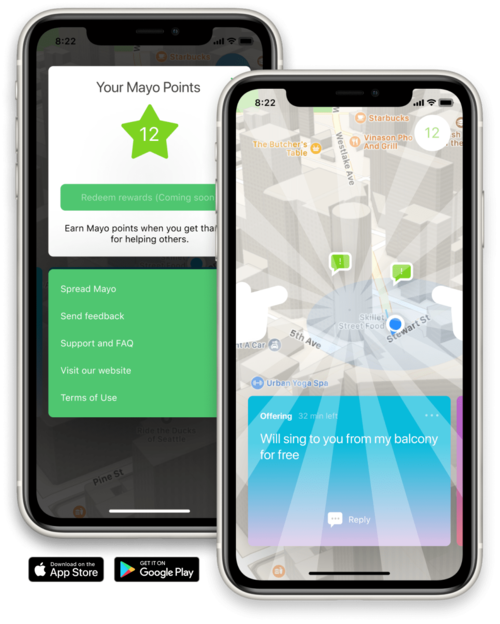
\includegraphics[scale=0.2]{slike/mayo-hero.PNG} %veličina slike u odnosu na originalnu datoteku i pozicija slike
	\centering
	\caption{Primjer konkurentne aplikacije}
\end{figure}

Zbog prirode naše aplikacije, samo će korisnici s napravljenim računom moći pregledati zahtjeve za pomoć i objaviti svoje.

\pagebreak
 Da bi korisnik napravio svoj račun, bit će potrebni:

\begin{packed_item}
	\item Korisničko ime
	\item E-mail adresa
	\item Zaporka
	\item Ime
	\item Prezime
	\item Preferirana lokacija
	\item Kontakt broj mobitela
	\item Datum rođenja
\end{packed_item}

Kada korisnik stvori svoj račun, omogućena mu je mogućnost prijave u aplikaciju unosom svojeg korisničkog imena i zaporke.

Prijavljenom korisniku sada se prikazuju zahtjevi za pomoć na početnom zaslonu, a pomoću intuitivnog korisničkog sučelja može postaviti svoj zahtjev za koji potražuje pomoć.

Opišimo sada kako će tipični korisnik navigirati našom aplikacijom.
Kada korisnik želi pomoći, odabire zahtjev s liste svih aktivnih zahtjeva
koji se nalaze unutar jednog kilometra od lokacije uređaja, pri čemu se lista može
proširiti na veće geografsko područje. Korisnik koji će provesti odabrani zahtjev
se smatra \textbf{izvršiteljem zahtjeva}. Valja napomenuti kako je svaka lista sortirana po određenom redoslijedu i omogućeno je
filtriranje zahtjeva prema kategorijama.\\
Kada traži pomoć, govorimo o ulozi \textbf{autora zahtjeva}. Prilikom zadavanja, autor unosi opis i kontakt podatke poput broja mobitela, adrese (opcionalno) i datum i/ili vrijeme do kada se zahtjev treba izvršiti (opcionalno).//
Budući da se više mogućih izvršitelja može javiti na jedan zahtjev, odabir onog konačnog vrši se metodom trostrukog rukovanja. To ćemo najbolje razjasniti primjerom: 

	\begin{packed_item}
	\item \textit {Teta Marica želi da joj netko donese 3kg krumpira (autor zahtjeva).}
	
	\item \textit {Ante i Marko vide da teta Marica treba pomoć i jave se na zahtjev (mogući izvršitelji).}
	\item \textit {Marica vidi da su se obojica javila, ali recimo da je Ante bolje ocijenjen i njega odabere (Ante je izvršitelj).}
	\end{packed_item}
	Kada je izvršitelj odabran, razmjenjuju se kontakt informacije i kreće proces izvršenja koji ostavljamo gore navedenim.
	
	Postavlja se pitanje kako je teta Marica znala da je Ante "bolji" izvršitelj? Zahvaljujući sustavu međusobnog ocjenjivanja korisnika! Po izvršenju zahtjeva autor označava da je zahtjev izvršen nakon čega se korisnici međusobno ocjenjuju ocjenama od 1-5 te opcionalno upisuju komentare. Kako novi korisnici ne bi ostali zakinuti za povjerenje budućih autora zahtjeva, ocjenjivanje bilo kojeg korisnika aplikacije moguće je u bilo kojem trenutku (ne samo nakon izvršenja zadatka) i ocjene se vide u detaljima profila, kao i komentari. Također, moguće je vidjeti i
	"lance povjerenja": da je korisnik kojeg ste vi visoko ocijenili ocijenio korisnika
	čiji profil gledate.
	
	Kako bi se čovjek mogao prisjetiti svoje i tuđe humanosti, svaki korisnik može vidjeti listu zahtjeva koje je zadao i izvršio. Sustav
	omogućuje i dodatne izvještaje/preglede, posebno one koji omogućuju
	kandidiranje za najboljeg pomagača godine.
	
	Da bismo zajednicu učinili sigurnijom, uveli smo ulogu \textbf{administratora}. Administratori se brinu oko sadržaja koji se objavljuje; imaju ovlasti
	brisanja zahtjeva koji se smatra opasnim, nemogućim, lažnim ili neetičkim te
	privremenog i trajnog blokiranja svih korisnika aplikacije. Administratori se
	dodjeljuju prema geografskim lokacijama. 
	
	Na kraju ovog opisa treba spomenuti nekoliko posebnosti. Ukoliko korisnik tijekom registracije ne želi unijeti svoju lokaciju, bit će mu vidljivi samo aktivni zahtjevi koji su označeni kao virtualni. Sjetimo se čovjeka koji je tražio pomoć oko namještanja postavki pisača, taj zahtjev je razumno označiti kao virtualni.
	Također, kako naša spomenuta teta Marica ne bi morala uvijek unositi adresu kada stvara novi zahtjev, adresa zahtjeva može se povući iz adrese s kojom je registrirana i tako Marici uštedjeti nekoliko sekundi svakim zahtjevom.
\eject



	\chapter{Specifikacija programske potpore}
		
	\section{Funkcionalni zahtjevi}
			
			\textbf{\textit{dio 1. revizije}}\\
			
			\textit{Navesti \textbf{dionike} koji imaju \textbf{interes u ovom sustavu} ili  \textbf{su nositelji odgovornosti}. To su prije svega korisnici, ali i administratori sustava, naručitelji, razvojni tim.}\\
				
			\textit{Navesti \textbf{aktore} koji izravno \textbf{koriste} ili \textbf{komuniciraju sa sustavom}. Oni mogu imati inicijatorsku ulogu, tj. započinju određene procese u sustavu ili samo sudioničku ulogu, tj. obavljaju određeni posao. Za svakog aktora navesti funkcionalne zahtjeve koji se na njega odnose.}\\
			
			
			\noindent \textbf{Dionici:}
			
			\begin{packed_enum}
				
				\item Dionik 1
				\item Dionik 2				
				\item ...
				
			\end{packed_enum}
			
			\noindent \textbf{Aktori i njihovi funkcionalni zahtjevi:}
			
			
			\begin{packed_enum}
				\item  \underbar{Aktor 1 (inicijator) može:}
				
				\begin{packed_enum}
					
					\item funkcionalnost 1
					\item funkcionalnost 2
					\begin{packed_enum}
						
						\item  podfunkcionalnost 1 
						\item  podfunkcionalnost 2
				
					\end{packed_enum}
					\item  funkcionalnost 3
					
				\end{packed_enum}
			
				\item  \underbar{Aktor 2 (sudionik) može:}
				
				\begin{packed_enum}
					
					\item funkcionalnost 1
					\item funkcionalnost 2
					
				\end{packed_enum}
			\end{packed_enum}
			
			\eject 
			
			
				
			\subsection{Obrasci uporabe}
				
				\textbf{\textit{dio 1. revizije}}
				
				\subsubsection{Opis obrazaca uporabe}
					\textit{Funkcionalne zahtjeve razraditi u obliku obrazaca uporabe. Svaki obrazac je potrebno razraditi prema donjem predlošku. Ukoliko u nekom koraku može doći do odstupanja, potrebno je to odstupanje opisati i po mogućnosti ponuditi rješenje kojim bi se tijek obrasca vratio na osnovni tijek.}\\
					

					\noindent \underbar{\textbf{UC1 - Pregled liste aktivnih zahtjeva}}
					\begin{packed_item}
	
						\item \textbf{Glavni sudionik: }Korisnik
						\item  \textbf{Cilj:} Pregledati aktivne zahtjeve za pomoć
						\item  \textbf{Sudionici:} Baza podataka
						\item  \textbf{Preduvjet:} Korisnik je prijavljen u sustav
						\item  \textbf{Opis osnovnog tijeka:}
						
						\item[] \begin{packed_enum}
	
							\item Prikaz liste aktivnih zahtjeva udaljenih od korisnikove adrese za zadani radius 
							\item Korisnik može odabrati alternativni radius
							\item Odabir pojedinog zahtjeva
							\item Prikaz detalja o odabranom zahtjevu
						\end{packed_enum}
						
						\item  \textbf{Opis mogućih odstupanja:}
						
						\item[] \begin{packed_item}
	
							\item[1.a] Zahtjev nema unesenu lokaciju
							\item[] \begin{packed_enum}
								
								\item Zahtjevi bez lokacije prikazuju se svim korisnicima
							
							\end{packed_enum}
							
							
						\end{packed_item}
					\end{packed_item}
				
				\noindent \underbar{\textbf{UC1.1 - Javljanje na zahtjev}}
				\begin{packed_item}
					
					\item \textbf{Glavni sudionik: }Korisnik
					\item  \textbf{Cilj:} Inicijalizirati komunikaciju s korisnikom autorom
					\item  \textbf{Sudionici:} Korisnik autor zahtjeva, Baza podataka
					\item  \textbf{Preduvjet:} Oglas je aktivan
					\item  \textbf{Opis osnovnog tijeka:}
					
					\item[] \begin{packed_enum}
						
						\item Korisnik odabire zahtjev
						\item Korisnik se uvodi u bazu podataka kao potencijalni izvršitelj za odabrani zahtjev
						\item Korisniku autoru dolazi obavijest o novom potencijalnom izvršitelju
					\end{packed_enum}
					
					\item  \textbf{Opis mogućih odstupanja:}
					
					\item[] \begin{packed_item}
						
						\item[1.a] Korisnik autor može biti blokiran
						\item[] \begin{packed_enum}
							
							\item Zahtjevi blokiranih korisnika ne prikazuju se na glavnoj stranici zahtjeva
							\item Zahtjevi blokiranih korisnika vidljivi na njegovom profilu ne mogu biti odabrani za izvršavanje
							
						\end{packed_enum}
						
						
					\end{packed_item}
				\end{packed_item}
				
				
				\noindent \underbar{\textbf{UC1.2 - Filtriranje zahtjeva}}
				\begin{packed_item}
					
					\item \textbf{Glavni sudionik: }Korisnik
					\item  \textbf{Cilj:} Primjeniti različite filtre na zahtjeve
					\item  \textbf{Sudionici:}-
					\item  \textbf{Preduvjet:} Korisnik je prijavljen
					\item  \textbf{Opis osnovnog tijeka:}
					
					\item[] \begin{packed_enum}
						
						\item Korisnik otvara odabir filtera
						\item Korisnik označava željene filtre
						\item Potvrđivanje označenih filtera
						\item Prikaz filtriranih zahtjeva 
						\item Korisnik može poništiti sve primjenjene filtre
					\end{packed_enum}
					
					\item  \textbf{Opis mogućih odstupanja:}
					
					\item[] \begin{packed_item}
						
						\item[4.a] Nema zahtjeva za prikaz
						\item[] \begin{packed_enum}
							
							\item Prikazuje se odgovarajuća poruka
							
						\end{packed_enum}
						
						
					\end{packed_item}
				\end{packed_item}
			
			\noindent \underbar{\textbf{UC1.3 - Promjena lokacije izvršenja}}
			\begin{packed_item}
				
				\item \textbf{Glavni sudionik: }Korisnik
				\item  \textbf{Cilj:}Jednostavna izmjena korisnikove lokacije
				\item  \textbf{Sudionici:} Baza podataka
				\item  \textbf{Preduvjet:} Korisnik je prijavljen
				\item  \textbf{Opis osnovnog tijeka:}
				
				\item[] \begin{packed_enum}
					
					\item Korisnik odabire izmjenu lokacije
					\item Korisnik unosi novu lokaciju tekstom ili odabirom na karti
					\item Nova lokacija pohranjuje se u bazu
					\item Prikaz zahtjeva u odnosu na novu lokaciju
				\end{packed_enum}
				
				\item  \textbf{Opis mogućih odstupanja:}
				
				\item[] \begin{packed_item}
					
					\item[2.a] Unos nevaljane lokacije
					\item[] \begin{packed_enum}
						
						\item Unos lokacije u bazu se stornira
						\item Korisniku se prikazuje odgovarajuća poruka
						
					\end{packed_enum}
				
					
				\end{packed_item}
			\end{packed_item}
			
			
	
			\noindent \underbar{\textbf{UC2 - Registracija}}
			\begin{packed_item}
				
				\item \textbf{Glavni sudionik: }Javni korisnik
				\item  \textbf{Cilj:} Stvoriti račun u aplikaciji
				\item  \textbf{Sudionici:} Baza podataka
				\item  \textbf{Preduvjet:} -
				\item  \textbf{Opis osnovnog tijeka:}
				
				\item[] \begin{packed_enum}
					
					\item Korisnik unosi potrebne podatke
					\item Potvrda unesenih podataka
					\item Upis podataka u bazu
					\item Nakon uspješne registracije korisnik se preusmjerava na stranicu zahtjeva
				\end{packed_enum}
				
				\item  \textbf{Opis mogućih odstupanja:}
				
				\item[] \begin{packed_item}
					
					\item[1.a] Korisnik unosi već zauzeto korisničko ime i/ili e-mail
					\item[] \begin{packed_enum}
						
						\item Prikaz odgovarajuće poruke
						\item Omogućavanje ponovnog unosa neodgovarajućih podataka
						
					\end{packed_enum}
					\item[1.b] Nisu popunjena sva obavezna polja
					\item[] \begin{packed_enum}
						
						\item Prikaz odgovarajuće poruke
						\item Omogućavanje ponovnog unosa podataka
						
					\end{packed_enum}
					\item[4.a] Mogućnost odustajanja od registracije klikom na gumb
					
				\end{packed_item}
			\end{packed_item}
		
			\noindent \underbar{\textbf{UC3 - Zadavanje novog zahtjeva}}
			\begin{packed_item}
				
				\item \textbf{Glavni sudionik: }Korisnik
				\item  \textbf{Cilj:} Unijeti i opisati svoj zahtjev za pomoć
				\item  \textbf{Sudionici:} Baza podataka
				\item  \textbf{Preduvjet:} Korisnik je prijavljen
				\item  \textbf{Opis osnovnog tijeka:}
				
				\item[] \begin{packed_enum}
					
					\item Korisnik otvara komponentu za unos zahtjeva
					\item Unos opisa zahtjeva
					\item Unos vremena isteka
					\item Potvrda zahtjeva
					\item Unos zahtjeva u bazu podataka
				\end{packed_enum}
				
				\item  \textbf{Opis mogućih odstupanja:}
				
				\item[] \begin{packed_item}
					
					\item[2.a] Unos zahtjeva sa praznim opisom
					\item[] \begin{packed_enum}
						
						\item Prikaz poruke o minimalnoj duljini opisa od dva znaka
						
					\end{packed_enum}
					
				\end{packed_item}
			\end{packed_item}
		
		
			\noindent \underbar{\textbf{UC3.1 - Odabir lokacije zahtjeva}}
			\begin{packed_item}
				
				\item \textbf{Glavni sudionik: }Korisnik
				\item  \textbf{Cilj:} Opcionalan odabir lokacije zahtjeva
				\item  \textbf{Sudionici:} Baza podataka
				\item  \textbf{Preduvjet:} U tijeku je zadavanje novog zahtjeva
				\item  \textbf{Opis osnovnog tijeka:}
				
				\item[] \begin{packed_enum}
					
					\item Korisnik se odlučuje za postavljanje lokacije
					\item Odabir ručnog unosa ili unosa na karti
					\item Otvaranje polja ili karte za unos lokacije
					\item Potvrda lokacije
					\item Nastavak zadavanja zahtjeva
				\end{packed_enum}
				
				\item  \textbf{Opis mogućih odstupanja:}
				
				\item[] \begin{packed_item}
					
					\item[3.a] Unos prazne lokacije
					\item[] \begin{packed_enum}
						
						\item Zahtjevi bez lokacije vode se kao virtualni i prikazuju se svim korisnicima
						\item Virtualni zahtjevi polaze od pretpostavke da je lokacija irelevantna za uspješno izvršavanje
						
					\end{packed_enum}
					
					
				\end{packed_item}
			\end{packed_item}
		
		
			\noindent \underbar{\textbf{UC4 - Pregled vlastitog profila}}
			\begin{packed_item}
				
				\item \textbf{Glavni sudionik: }Korisnik
				\item  \textbf{Cilj:} Pregled vlasititih informacija i zahtjeva na profilu
				\item  \textbf{Sudionici:} -
				\item  \textbf{Preduvjet:} Korisnik je prijavljen
				\item  \textbf{Opis osnovnog tijeka:}
				
				\item[] \begin{packed_enum}
					
					\item Korisnik odabire opciju za prikaz profila
					\item Korisnik pregledava vlastite aktivne i izvršene zahtjeve
					\item Pregled vlastitih podataka korisničkog računa
				\end{packed_enum}
				
				
			\end{packed_item}
		
		
			\noindent \underbar{\textbf{UC4.1 - Upravljanje korisničkim podacima}}
			\begin{packed_item}
				
				\item \textbf{Glavni sudionik: }Korisnik
				\item  \textbf{Cilj:} Aktualizacija i izmjena 
				\item  \textbf{Sudionici:} Baza podataka
				\item  \textbf{Preduvjet:} Korisnik je prijavljen
				\item  \textbf{Opis osnovnog tijeka:}
				
				\item[] \begin{packed_enum}
					
					\item Korisnik odabire opciju izmjene podataka korisničkog računa
					\item Unos novih podataka
					\item Potvrda izmjena
					\item Spremanje izmjena u bazu podataka
				\end{packed_enum}
				
				\item  \textbf{Opis mogućih odstupanja:}
				
				\item[] \begin{packed_item}
					
					\item[3.a] Unos podataka u krivom formatu ili neispunjenje obaveznih polja
					\item[] \begin{packed_enum}
						
						\item Prikaz odgovarajuće poruke
						\item Ponovna mogućnost unosa podataka
						
					\end{packed_enum}
					
				\end{packed_item}
			\end{packed_item}
		
		
			\noindent \underbar{\textbf{UC4.3 - Brisanje korisničkog računa}}
			\begin{packed_item}
				
				\item \textbf{Glavni sudionik: }Korisnik
				\item  \textbf{Cilj:} Brisanje korisničkog računa i pratećih podataka 
				\item  \textbf{Sudionici:} Baza podataka
				\item  \textbf{Preduvjet:} -
				\item  \textbf{Opis osnovnog tijeka:}
				
				\item[] \begin{packed_enum}
					
					\item Odabir opcije brisanja korisničkog računa
					\item Korisnik mora dvostruko potvrditi akciju brisanja
					\item Korisnik u svakom trenutku prije finalne potvrde može odustati od brisanja
					\item Brisanje korisnika i popratnih podataka iz baze
				\end{packed_enum}
				
				
			\end{packed_item}
		
			\noindent \underbar{\textbf{UC4.4 - Pregled javljanja na zahtjeve}}
			\begin{packed_item}
				
				\item \textbf{Glavni sudionik: }Korisnik
				\item  \textbf{Cilj:} Pregled i pristup zahtjevima na koje se korisnik javio kao potencijalni izvršitelj 
				\item  \textbf{Sudionici:} Baza podataka
				\item  \textbf{Preduvjet:} -
				\item  \textbf{Opis osnovnog tijeka:}
				
				\item[] \begin{packed_enum}
					
					\item Korisnik odabire opciju prikaza zahtjeva na koje se javio
					\item Prikazuju se zahtjevi gdje je korisnik u listi potencijalnih izvršitelja

				\end{packed_enum}
				
				\item[1.b] Zahtjev za koji se korisnik javio je blokiran
				\item[] \begin{packed_enum}
					
					\item Blokirani zahtjevi se ne mogu izvršavati i ne prikazuju se među korisnikovim javljanjima na zahtjev
					
				\end{packed_enum}
					
				
			\end{packed_item}
		
	
			\noindent \underbar{\textbf{UC5 - Pregled statistike}}
			\begin{packed_item}
				
				\item \textbf{Glavni sudionik: }Korisnik
				\item  \textbf{Cilj:} Prikaz statistika o korisnicima 
				\item  \textbf{Sudionici:} Baza podataka
				\item  \textbf{Preduvjet:} -
				\item  \textbf{Opis osnovnog tijeka:}
				
				\item[] \begin{packed_enum}
					
					\item Korisnik odabire opciju prikaza statistika
					\item Prikaz statistike u aplikaciji
					\item Povratak na prethodnu stranicu
			
				\end{packed_enum}
				
				
				
			\end{packed_item}
		
			\noindent \underbar{\textbf{UC6 - Pregled potencijalnih izvršitelja}}
			\begin{packed_item}
				
				\item \textbf{Glavni sudionik: }Korisnik
				\item  \textbf{Cilj:} Prikazati korisnike koji su se javili na pojedini zahtjev 
				\item  \textbf{Sudionici:} Baza podataka
				\item  \textbf{Preduvjet:} Postoje vlastiti aktivni zahtjevi
				\item  \textbf{Opis osnovnog tijeka:}
				
				\item[] \begin{packed_enum}
					
					\item Korisnik na zahtjevu bira opciju za prikaz potencijalnih izvršitelja
					\item Prikaz potencijalnih izvršitelja s opcijama za prihvaćanje i odbijanja
				\end{packed_enum}
				
				\item  \textbf{Opis mogućih odstupanja:}
				
				\item[] \begin{packed_item}
					
					\item[2.a] Odabrani zahtjev nema potencijalnih izvršitelja
					\item[] \begin{packed_enum}
						
						\item Prikaz poruke o nepostojanju potencijalnih izvršitelja
						
					\end{packed_enum}
					
				\end{packed_item}
			\end{packed_item}
		
			\noindent \underbar{\textbf{UC6.1 - Prihvaćanje javljanja na zahtjev}}
			\begin{packed_item}
				
				\item \textbf{Glavni sudionik: }Korisnik
				\item  \textbf{Cilj:} Prihvaćanje javljanja na zahtjev za pomoć 
				\item  \textbf{Sudionici:} Korisnik izvršitelj
				\item  \textbf{Preduvjet:} Postoji barem jedan potencijalni izvršitelj za zahtjev, Zahtjev je aktivan
				\item  \textbf{Opis osnovnog tijeka:}
				
				\item[] \begin{packed_enum}
					
					\item Prikaz liste potencijalnih izvršitelja
					\item Korisnik prihvaća pojedino javljanje na zahtjev
					\item Slanje obavijesti prihvaćenom korisniku
					\item Odbijanje ostalih potencijalnih izvršitelja
					\item Slanje obavijesti odbijenim korisnicima
					\item Pražnjenje liste potencijalnih izvršitelja
					\item Dodavanje prihvaćenog korisnika kao izvršitelja zahtjeva
				\end{packed_enum}
				
			\end{packed_item}
		
			\noindent \underbar{\textbf{UC6.2 - Odbijanje javljanja na zahtjev}}
			\begin{packed_item}
				
				\item \textbf{Glavni sudionik: }Korisnik
				\item  \textbf{Cilj:} Odbijanje pojedinog ili više potencijalnih izvršitelja
				\item  \textbf{Sudionici:} Korisnik izvršitelj
				\item  \textbf{Preduvjet:} Postoji barem jedan potencijalni izvršitelj za zahtjev
				\item  \textbf{Opis osnovnog tijeka:}
				
				\item[] \begin{packed_enum}
					
					\item Prikaz liste potencijalnih izvršitelja
					\item Korisnik odbija pojedino javljanje na zahtjev
					\item Odbijenom korisniku šalje se obavijest o odbijanju
				\end{packed_enum}
				
			\end{packed_item}
		
			\noindent \underbar{\textbf{UC7 - Administriranje korisnika}}
			\begin{packed_item}
				
				\item \textbf{Glavni sudionik: }Administrator
				\item  \textbf{Cilj:} Omogućiti rukovanje korisnicima 
				\item  \textbf{Sudionici:} Korisnici, Baza podataka
				\item  \textbf{Preduvjet:} -
				\item  \textbf{Opis osnovnog tijeka:}
				
				\item[] \begin{packed_enum}
					
					\item Na profilu korisnika administrator odabire opciju administriranja korisnika
					\item Administrator bira opciju privremenog blokiranja ili brisanja korisnika
					\item Administrator potvrđuje odabir
					\item Unos blokiranja/brisanja u bazu podataka
				\end{packed_enum}
				
			\end{packed_item}
		
		
			\noindent \underbar{\textbf{UC8 - Dodavanje novog administratora}}
			\begin{packed_item}
				
				\item \textbf{Glavni sudionik: }Administrator
				\item  \textbf{Cilj:} Postaviti nekog korisnika kao administratora 
				\item  \textbf{Sudionici:} Baza Podataka
				\item  \textbf{Preduvjet:} -
				\item  \textbf{Opis osnovnog tijeka:}
				
				\item[] \begin{packed_enum}
					
					\item Administrator na profilu korisnika odabire opciju postavljanja administratorskih ovlasti
					\item Administrator potvrđuje odabir
					
				\end{packed_enum}
				
				\item  \textbf{Opis mogućih odstupanja:}
				
				\item[] \begin{packed_item}
					
					\item[1.a] Pregledavanje profila korisnika koji već ima dodjeljene administratorske ovlasti
					\item[] \begin{packed_enum}
						
						\item Administratoru se ne omogućava ponovo postavljanje ovlasti
						
					\end{packed_enum}
					
				\end{packed_item}
			\end{packed_item}
		
			\noindent \underbar{\textbf{UC9 - Administriranje zahtjeva}}
			\begin{packed_item}
				
				\item \textbf{Glavni sudionik: }Administrator
				\item  \textbf{Cilj:} Brisanje neprihvatljivih zahtjeva 
				\item  \textbf{Sudionici:} Baza podataka
				\item  \textbf{Preduvjet:} -
				\item  \textbf{Opis osnovnog tijeka:}
				
				\item[] \begin{packed_enum}
					
					\item Administrator odabire opciju brisanja zahtjeva
					\item Administrator potvrđuje odabir
					\item Autoru zahtjeva dolazi obavijest o brisanju zahtjeva
					\item Potencijalnim izvršiteljima se šalje obavijest o brisanju zahtjeva
				\end{packed_enum}
				
				\item  \textbf{Opis mogućih odstupanja:}
				
				\item[] \begin{packed_item}
					
					\item[2.a] Javljanje na zahtjev je već prihvaćeno i izvršitelj je postavljen
					\item[] \begin{packed_enum}
						
						\item Izvršitelj dobiva obavijest o brisanju zahtjeva
						
					\end{packed_enum}
					
				\end{packed_item}
			\end{packed_item}
		
		
			\noindent \underbar{\textbf{UC10 - Pregled profila drugih korisnika}}
			\begin{packed_item}
				
				\item \textbf{Glavni sudionik: }Korisnik
				\item  \textbf{Cilj:} Pregled profila korisnika 
				\item  \textbf{Sudionici:} -
				\item  \textbf{Preduvjet:} -
				\item  \textbf{Opis osnovnog tijeka:}
				
				\item[] \begin{packed_enum}
					
					\item Prikaz osnovnih podataka o korisniku, njegovih zahtjeva i zahtjeva koje je on izvršio
					\item Korisnik može pregledavati zahtjeve profila
					\item Korisnik može pregledati lanac povjerenja, komentare i ocjenu profila korisnika
				\end{packed_enum}
				
			\end{packed_item}
		
		
			\noindent \underbar{\textbf{UC11 - Ocjenjivanje korisnika}}
			\begin{packed_item}
				
				\item \textbf{Glavni sudionik: }Korisnik
				\item  \textbf{Cilj:} Ocjena korisnika i/ili ocjena izvršenja zahtjeva uz popratan komentar 
				\item  \textbf{Sudionici:} Baza podataka
				\item  \textbf{Preduvjet:} -
				\item  \textbf{Opis osnovnog tijeka:}
				
				\item[] \begin{packed_enum}
					
					\item Korisnik inicira ocjenjivanje na profilu ili se ocjenjivanje pokreće nakon izvršenja zahtjeva
					\item Korisnik izabire ocjenu od 1 do 5
					\item Korisnik opcionalno unosi komentar
					\item Korisnik potvrđuje svoj odabir
					\item Ocjena i komentar se
				\end{packed_enum}
				
				\item  \textbf{Opis mogućih odstupanja:}
				
				\item[] \begin{packed_item}
					
					\item[2.a] Ocjena se može, ali ne mora odnositi na izvršavanje specifičnog zahtjeva
					\item[] \begin{packed_enum}
						
						\item Ukoliko se ocjena odnosi na izvršavanje zahtjeva, u bazu se upisuje o kojem se zahtjevu radi
						
					\end{packed_enum}
					
				\end{packed_item}
			\end{packed_item}
		
		
			\noindent \underbar{\textbf{UC12 - Izvršavanje zahtjeva}}
			\begin{packed_item}
				
				\item \textbf{Glavni sudionik: }Korisnik
				\item  \textbf{Cilj:} Označavanje zahtjeva izvršenim 
				\item  \textbf{Sudionici:} Baza podataka
				\item  \textbf{Preduvjet:} Korisnik je postavljen kao izvršitelj zahtjeva
				\item  \textbf{Opis osnovnog tijeka:}
				
				\item[] \begin{packed_enum}
					
					\item Korisnik odabire zahtjev koji izvršava
					\item Korisnik označuje zahtjev izvršenim
					\item Korisniku autoru šalje se obavijest o izvršenju
					\item Inicira se ocjenjivanje korisnika

				\end{packed_enum}
			
				\item[1.a] Zahtjev je istekao prije nego što je korisnik potvrdio izvršenje
				\item[] \begin{packed_enum}
					
					\item Zahtjevi za koje je korisnik odabran kao izvršitelj prikazuju se unatoč istjecanju i mogu se odabrati za izvršavanje
					
				\end{packed_enum}
				\item[1.b] Zahtjev za koji je korisnik odabran kao izvršitelj je blokiran
				\item[] \begin{packed_enum}
					
					\item Blokirani zahtjevi se ne mogu izvršavati i ne prikazuju se među korisnikovim zahtjevima za izvršavanje
					
				\end{packed_enum}
					
				
			\end{packed_item}
		
		
			\noindent \underbar{\textbf{UC13 - Prijava u sustav}}
			\begin{packed_item}
				
				\item \textbf{Glavni sudionik: }Javni korisnik
				\item  \textbf{Cilj:} Aktualizacija i izmjena 
				\item  \textbf{Sudionici:} -
				\item  \textbf{Preduvjet:} Javni korisnik ima izrađen korisnični račun u sustavu
				\item  \textbf{Opis osnovnog tijeka:}
				
				\item[] \begin{packed_enum}
					
					\item Javni korisnik odabire opciju prijave
					\item Javni korisnik upisuje korisničko ime i lozinku
					\item Korisnik potvrđuje unos
				\end{packed_enum}
				
				\item  \textbf{Opis mogućih odstupanja:}
				
				\item[] \begin{packed_item}
					
					\item[2.a] Unos pogrešnog korisničkog imena i/ili lozinke
					\item[] \begin{packed_enum}
						
						\item Javnom korisniku ispisuje se poruka o pogrešci lozinke ili korisničkog imena
						
					\end{packed_enum}
					
					
				\end{packed_item}
			\end{packed_item}
		
		
			\noindent \underbar{\textbf{UC14 - Odjava}}
			\begin{packed_item}
				
				\item \textbf{Glavni sudionik: }Korisnik
				\item  \textbf{Cilj:} Odjava iz sustava 
				\item  \textbf{Sudionici:} -
				\item  \textbf{Preduvjet:} Korisnik je prijavljen u sustav
				\item  \textbf{Opis osnovnog tijeka:}
				
				\item[] \begin{packed_enum}
					
					\item Korisnik odabire opciju odjave
					\item Korisnik se preusmjerava na stranicu za prijavu
				\end{packed_enum}
				
			\end{packed_item}
		
			
		
			\noindent \underbar{\textbf{UC15 - Upravljanje vlastitim zahjevima}}
			\begin{packed_item}
				
				\item \textbf{Glavni sudionik: }Korisnik
				\item  \textbf{Cilj:} Mogućnost izmjene, brisanja ili blokiranja vlastitih zahtjeva
				\item  \textbf{Sudionici:} Baza podataka
				\item  \textbf{Preduvjet:} -
				\item  \textbf{Opis osnovnog tijeka:}
				
				\item[] \begin{packed_enum}
					
					\item Korisnik odabire vlastiti zahtjev kojim želi upravljati
					\item Korisnik odabire izmjenu, brisanje ili blokiranje zahtjeva
					\item Ukoliko je odabrana izmjena, unose se novi podaci 
					\item Korisnik potvrđuje odabir

				\end{packed_enum}
				
				\item  \textbf{Opis mogućih odstupanja:}
				
				\item[] \begin{packed_item}
					
					
					\item[2.a] Na zahtjev se netko već javio, postoje potencijalni izvršitelji
					\item[] \begin{packed_enum}
						
						\item Zahtjevi na koje se netko već javio mogu se samo blokirati
						\item Prilikom blokiranja zahtjeva svim potencijalnim izvršiteljima se dostavlja obavijest o blokiranju zahtjeva
						
					\end{packed_enum}
					\item[3.a] Uneseni novi komentar je prazan
					\item[] \begin{packed_enum}
						
						\item Ispisuje se poruka korisniku o minimalnoj mogućoj duljini unesenog komentara
						
					\end{packed_enum}
										
				\end{packed_item}
			\end{packed_item}
		
					
					
				\subsubsection{Dijagrami obrazaca uporabe}
					
					\textit{Prikazati odnos aktora i obrazaca uporabe odgovarajućim UML dijagramom. Nije nužno nacrtati sve na jednom dijagramu. Modelirati po razinama apstrakcije i skupovima srodnih funkcionalnosti.}
				\eject		
				
			\subsection{Sekvencijski dijagrami}
				
				\textbf{\textit{dio 1. revizije}}\\
				
				\textit{Nacrtati sekvencijske dijagrame koji modeliraju najvažnije dijelove sustava (max. 4 dijagrama). Ukoliko postoji nedoumica oko odabira, razjasniti s asistentom. Uz svaki dijagram napisati detaljni opis dijagrama.}
				\eject
	
		\section{Ostali zahtjevi}
		
		\begin{itemize}
			\item Aplikacija treba biti izvedena kao web aplikacija prilagođena mobilnom uređaju.
			\item Sustav mora podržavati rad više korisnika u stvarnom vremenu.
			\item Sustav kao valutu koristi HRK.
			\item Procesiranje bilo kakve korisničke interakcije sa sustavom ne bi trebalo trajati duže od par sekundi.
			\item Administratori su dodijeljeni po geografskim lokacijama.
			\item Sustav mora podržavati hrvatske dijakritičke znakove.
			\item Informacije o zahtjevima moraju biti redovno ažurirane.
			\item U sustavu je potrebno registrirati barem 5 korisnika te 2 administratora.
			\item Korisničko sučelje treba biti jednostavno za korištenje.
		\end{itemize}
			 
			 
			 
	
	\chapter{Arhitektura i dizajn sustava}
			
			
			Odabir odgovarajuće arhitekture je važna odluka koja utječe na cjelokupnu funkcionalnost sustava. Budući da je cilj aplikacije široka dostupnost, odabrali smo web aplikaciju. Web aplikacija funkcionira neovisno o platformi, što oslobađa razvojni tim višeplatformnog razvoja.\\
			Korisnik aplikaciji pristupa pomoću web preglednika. Web preglednik je program koji omogućava korisniku pregled i prikaz web aplikacije na uređaju. Kako bi se omogućila komunikacija klijenta(korisnika) s aplikacijom koristi se web poslužitelj koji koristi HTTP protokol. Aplikacija komunicira sa backend-om preko REST API-ja. Backend dohvaća sve potrebne podatke iz baze podataka(više o njoj u sljedećoj sekciji) nakon čega preko poslužitelja i preglednika prikazuje te podatke korisniku u obliku HTML dokumenta.\\
			Aplikacija je pisana u programskom jeziku Java i programskom okruženju Spring Boot, te React-u(JavaScript biblioteka za izgradnju korisničkih sučelja), a od razvojnih okruženja odabrali smo Visual Studio Code za frontend  te IntelliJ IDEA za ostatak posla.\\
			
Logika backenda izgrađena je na temelju REST konvencije, stoga je razrađena u tri sloja: Repository, Service i Controller. 
			\begin{itemize}
				\item \textbf{Repository} – Sloj Repository primarno je zadužen za komunikaciju s bazom podataka. U njemu se nalaze standardne metode za dohvaćanje, spremanje i izmjenu podataka u bazi. Te metode temelje se na atributima entiteta za koji je izgrađen pojedini repository. Također, svaki repository može biti nadopunjen vlastitim metodama.
				\item \textbf{Service} – U Service sloju odvija se poslovna logika i manipulacija podacima koji dolaze s baze. To uključuje kreiranje klasa, promjenu tipova, omatanje i sl. 
				\item \textbf{Controller} –  prima i obrađuje zahtjeve poslužitelja. Svi se zahtjevi prosljeđuju koristeći JSON format. Shodno pojedinom zahtjevu, controller zatražuje podatke sa repositoryja, izvodi metode koje mu pruža Service. Na kraju podatke u obliku objekata šalje kao odgovor web poslužitelju.  
			\end{itemize}
			React je javascript knjižnica za izgradnju korisničkih sučelja. Temelji se na deklariranju komponenata koje se prikazuju korisniku preko web preglednika.
			\begin{figure}
				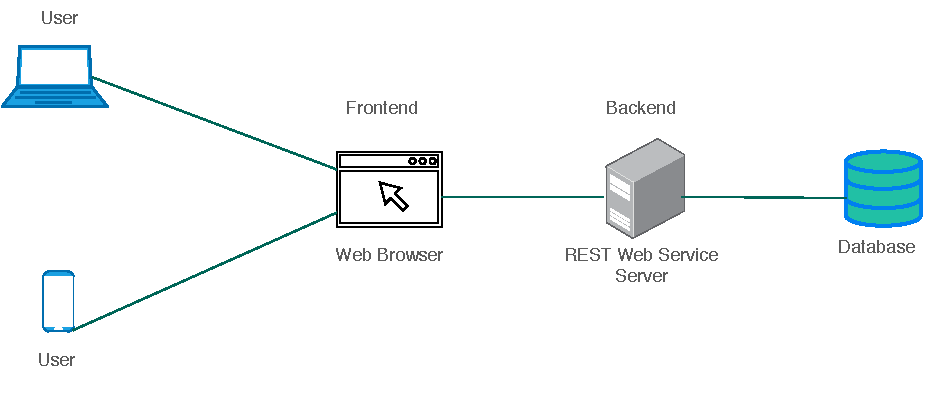
\includegraphics{Arhitektura_sustava}
				\caption{Arhitektura sustava}
			\end{figure}
			
			
			
			\section{Baza podataka}

			Sve je podatke potrebno negdje spremiti kako bi se mogli dinamički dohvaćati. Za ovo nam služi baza podataka, koju također smatramo dijelom MVC obrasca. Naša aplikacija u pozadini koristi, kao relacijsku bazu podataka, PostgreSQL.
			\\
			U bazi podataka nalaze se sljedeći entiteti:
			\begin{itemize}
				\item Korisnik
				\item Adresa
				\item Ocjena
				\item Zahtjev
				\item Obavijest
				\item Potencijalni
			\end{itemize}
			
			\subsection{Opis tablica}
			
			
			\textbf{Korisnik} Ovaj entitet modelira jednog korisnika aplikacije.\\
			Sadrži atribute: korisnikID, ime, prezime, e-posta, lozinka, korisnickoIme, jeAdmin, telefon, slika, status, i
			adresaID koji predstavlja strani ključ na entitet Adresa. Korisnik je povezan s entitetom Ocjena vezama "prima" i "daje" (\textit{One-to-Many}) preko atributa korisnikID. Korisnik se također veže s entitetom Zahtjev vezama "autorski" i "izvršiteljski" (\textit{One-to-Many}) preko atributa korisnikID i vezom "potencijalni" (\textit{Many-to-Many}) preko atributa korisnikID. Ovaj entitet se još veže uz entitet Adresa vezom \textit{Many-to-One} preko atributa adresaID. Također je u vezi s entitetom Obavijest vezom \textit{One-To-Many} preko atributa korisnikID.
			
			\begin{tabularx} {\textwidth} {|p{3.5cm}|p{2cm}|X|}
				
				\hline
				\multicolumn{3}{|c|}{\textbf{Korisnik}} \\
				\hline
				
				
				\cellcolor{LightGreen}korisnikID & INT	&   jedinstveni identifikator svakog korisnika 	\\ \hline
				ime	& VARCHAR &   ime korisnika	\\ \hline 
				prezime & VARCHAR &  prezime korisnika \\ \hline 
				e-posta & VARCHAR	&  	e-mail adresa korisnika	\\ \hline 
				lozinka & VARCHAR	&  	hash lozinke	\\ \hline
				korisnickoIme & VARCHAR	&  	korisnicko ime	\\ \hline
				jeAdmin & BOOLEAN	&  	oznaka je li korisnik administrator	\\ \hline
				telefon & VARCHAR	&  	broj mobitela korisnika	\\ \hline
				slika & BOOLEAN	&  	oznaka je li korisnik ima sliku profila	\\ \hline
				status & VARCHAR	&  	oznaka statusa korisničkog računa	\\ \hline
				\cellcolor{LightBlue}adresaId & VARCHAR	&  	adresa prebivališta korisnika	\\ \hline
				
				
				
			\end{tabularx} 
			
			\bigskip
			\bigskip
			\textbf{Adresa} Ovaj entitet modelira adresu prebivališta pojedinog korisnika aplikacije.
			Sadrži sljedeće atribute: adresaID, opis, xKoordinata, yKoordinata. Entitet Adresa je u vezi \textit{One-to-Many} s entitetom Zahtjev preko atributa adresaID i u vezi \textit{One-to-Many} s entitetom Korisnik pomoću atributa adresaID.
			\bigskip
			
			
			\begin{tabularx} {\textwidth} {|p{3.5cm}|p{2cm}|X|}
				
				\hline
				\multicolumn{3}{|c|}{\textbf{Adresa}} \\
				\hline
				
				\cellcolor{LightGreen}adresaID & INT	& jedinstveni identifikator adrese korisnika	\\ \hline 
				opis & VARCHAR & Detaljniji opis adrese korisnika  \\ \hline 
				xKoordinata & NUMERIC	& X koordinata adrese korisnika predočena na karti	\\ \hline 
				yKoordinata & NUMERIC	& Y koordinata adrese korisnika predočene na karti		\\ \hline
				
				
				
			\end{tabularx}
			
			\bigskip
			\bigskip
			\textbf{Ocjena} Ovaj entitet predstavlja ocjenu koju jedan korisnik daje drugome. Sadrži atribute: ocjenaID, komentar, ocjena, korisnikID, zahtjevID, primakorisnikID. Ovaj entite sadrži tri strana ključa, a to su: korisnikID(predstavlja korisnika koji ocjenjuje), primakorisnikID(predstavlja korisnika kojeg se ocjenjuje) i zahtjevID(predstavlja zahtjev koji se izvršava). Ocjena je u  dvije veze s entitetom Korisnik, a to su "prima" (\textit{Many-to-One}) i "daje" (\textit{Many-to-One}) preko atributa korisnikID. Ocjena se još veže uz Zahtjev vezom \textit{One-to-One} preko atributa zahtjevID. 
			\bigskip
			
			\begin{tabularx} {\textwidth} {|p{3.5cm}|p{2cm}|X|}
				
				\hline
				\multicolumn{3}{|c|}{\textbf{Ocjena}} \\
				\hline
				
				\cellcolor{LightGreen}ocjenaID & INT	& jedinstveni identifikator svake ocjene	\\ \hline
				komentar	& VARCHAR &  komentar kojeg korisnik ostavlja uz ocjenu 	\\ \hline 
				ocjena & INT & ocjena koju korisnik dodjeljuje  \\ \hline 
				\cellcolor{LightBlue} korisnikID	& INT &  korisnik koji ocjenjuje 	\\ \hline 
				\cellcolor{LightBlue} zahtjevID	& INT &  zahtjev koji se izvršava 	\\ \hline 
				\cellcolor{LightBlue} primakorisnikID	& INT &  korisnik kojeg se ocjenjuje 	\\ \hline 
				
			\end{tabularx}
			
			\bigskip
			\bigskip
			\textbf{Zahtjev} Ovaj entitet predstavlja jedan zahtjev kojeg korisnik aplikacije zadaje ili izvršava. Sadrži atribute:zahtjevID, opis, datumVrPocetka, naslov, datumIsteka, status, adresaID, korisnikID, autorskikorisnikID. Kao i entitet ocjena i ovaj entitet sadrži tri strana ključa: adresaID(predstavlja adresu korisnika koji je zadao zahtjev, nije obavezno kako bi se kreirao zahtjev), korisnikID(predstavlja izvršitelja zahtjeva) i autorskikorisnikID(predstavlja samog kreatora zahtjeva). Entitet je u vezi s Ocjenom preko veze \textit{One-to-One} pomoću atributa zahtjevID. Zahtjev se veže uz entitet Korisnik preko tri veze "autorski" (\textit{Many-to-One}), veze "izvršiteljski" (\textit{Many-to-One}) i veze "potencijalni" (\textit{Many-to-Many}) svaka preko atributa korisnikID. Još se veže uz entitet Adresa \textit{One-to-Many} preko atributa adresaID. Također je u vezi s entitetom Obavijest vezom \textit{One-To-Many} preko atributa zahtjveID. 
			\bigskip
			
			\begin{tabularx} {\textwidth} {|p{3.5cm}|p{2cm}|X|}
				
				\hline
				\multicolumn{3}{|c|}{\textbf{Zahtjev}} \\
				\hline
				
				\cellcolor{LightGreen}zahtjevID & INT	& jedinstveni identifikator svakog zahtjeva	\\ \hline
				opis	& VARCHAR &  opis zahtjeva 	\\ \hline 
				datumVrPocetka & DATETIME &  trenutak postavljanja zahtjeva na aplikaciju \\ \hline 
				datumIsteka & DATE	&  datum kada zahtjev istječe, te se ne može više izvršavati		\\ \hline
				naslov & VARCHAR	&  naslov zahtjeva
				\\
				\hline
				status & VARCHAR & status zahtjeva  \\ \hline
				\cellcolor{LightBlue} adresaID	& INT &  adresa autora zahtjeva 	\\ \hline 
				\cellcolor{LightBlue} korisnikID	& INT &  izvršitelj zahtjeva 	\\ \hline
				\cellcolor{LightBlue} autorskikorisnikID	& INT &   autor zahtjeva	\\ \hline
				
				
			\end{tabularx}
			
			\bigskip
			\bigskip
			\textbf{Potencijalni} Ovaj entitet predstavlja sve potencijalne izvršitelje jednog zahtjeva. Sadrži atribute: zahtjevID, korisnikID. Oba atributa su strani ključevi. Prvi predstavlja zahtjev kojeg korisnik želi izvršiti, drugi predstavlja korisnika koji želi izvršit zahtjev. Ovaj entitet nastaje radi \textit{Many-to-Many} veze "potencijalni" između Zahtjeva i Korisnika.
			\bigskip
			
			\begin{tabularx}{\textwidth} {|p{2cm}|p{2cm}|X|}
				\hline
				\multicolumn{3}{|c|}{\textbf{Potencijalni}} \\
				\hline
				\cellcolor{LightGreen} zahtjevID & INT & zahtjev kojeg korisnik želi izvršiti \\
				\hline
				\cellcolor{LightGreen} korisnikID & INT & potencijalni izvršitelj zahtjeva \\
				\hline
			\end{tabularx}
			
			\bigskip
			\bigskip
			\textbf{Obavijest} Ovaj entitet predstavlja sve moguće obavijesti koje jedan korisnik može dobiti. Sadrži atribute: obavijestID, korisnikID,
			poruka, zahtjevID, jeliPročitana. Ovaj entite sadrži dva strana ključa: korisnikID(predstavlja korisnika kojem je obavijest namijenjena), te zahtjevID(predstvavlja zahtjev na kojeg se obavijest odnosi). Entitet je u vezi s entitetom Korisnik vezom \textit{Many-To-One} pomoću atributa korisnikID, te s entitetom Zahtjev vezom \textit{Many-To-One} preko atributa zahtjevID.
			\bigskip
			
			\begin{tabularx}{\textwidth} {|p{2.4cm}|p{2cm}|X|}
				\hline
				\multicolumn{3}{|c|}{\textbf{Obavijest}} \\
				\hline
				\cellcolor{LightGreen} obavijestID & INT & jedinstveni identifikator obavijesti \\
				\hline
				poruka & VARCHAR & predstavlja detaljniji opis obavijesti \\
				\hline
				jeliPročitana & BOOLEAN & označuje jeli korisnik pročitao obavijest \\
				\hline
				\cellcolor{LightBlue}
				korisnikID & INT & korisnik kojem je obavijest namijenjena. \\
				\hline
				\cellcolor{LightBlue}
				zahtjevID & INT & zahtjev na kojeg se obavijest odnosi \\
				\hline
			\end{tabularx}
			
			
			
			\newpage
			\subsection{Dijagram baze podataka}
			Podcrtani elementi su ključevi, elementi koji imaju (O) nisu obavezni za unos u bazu podataka, elementi koji imaju (FK) su strani ključevi i elementi s oznakom (U) moraju biti jedinstveni.
			
			\begin{figure}[h]
				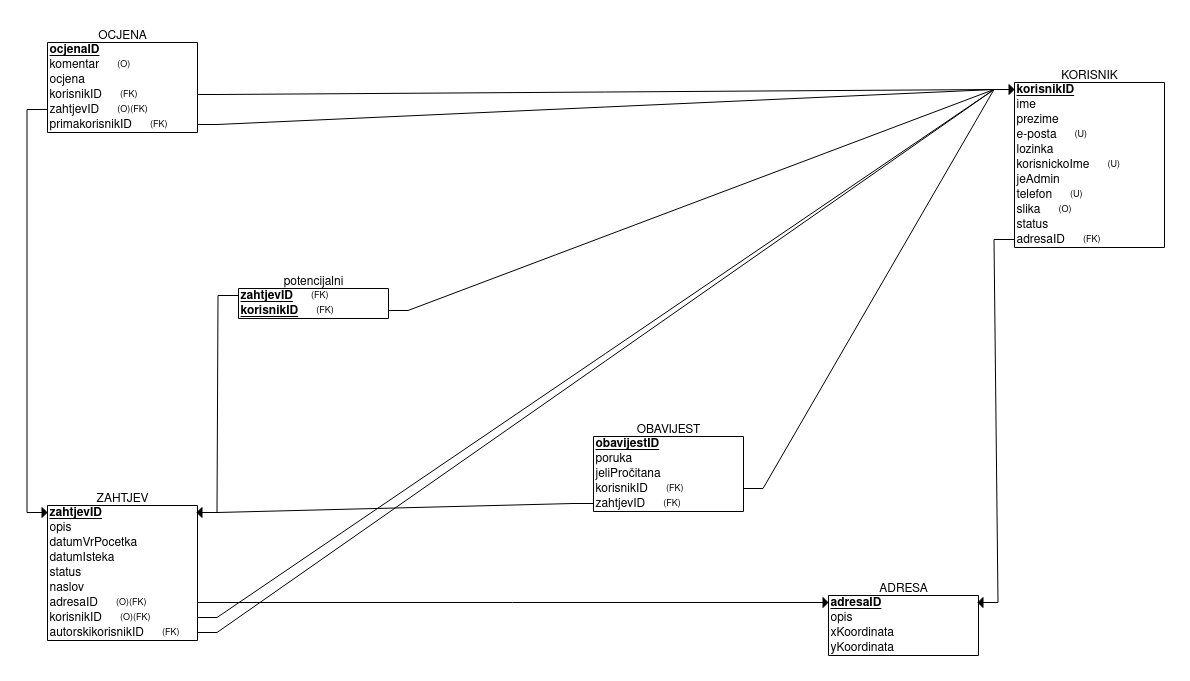
\includegraphics[height=0.45\textheight]{Relacijski_model}
				\caption{Relacijski model baze podataka}
			\end{figure}
			
			\eject
			


			
			
		\section{Dijagram razreda}
		
			U ovom poglavlju opisana je struktura \textit{backenda} aplikacije te opisana glavna funkcionalnost pojedinih klasa.\newline
			\newline
		
		
		
				Na slici 4.3 prikazana je konfiguracija aplikacije \textit{Pomozi mi}. Konfiguracija aplikacije temelji se na postavkama u klasi \textit{WebSecurity}, kojom su definiranja dopuštenja pristupa za pojedini \textit{path}, ponašanje pri \textit{loginu} i \textit{logoutu}. \\
				Klasom RestExceptionHandler regulirano je ponašanje sustava pri pojavi iznimke. Pojava iznimki rezultira \textit{responseom} u kojem je sadržana poruka iznimke.
				
				\begin{figure}[H]
					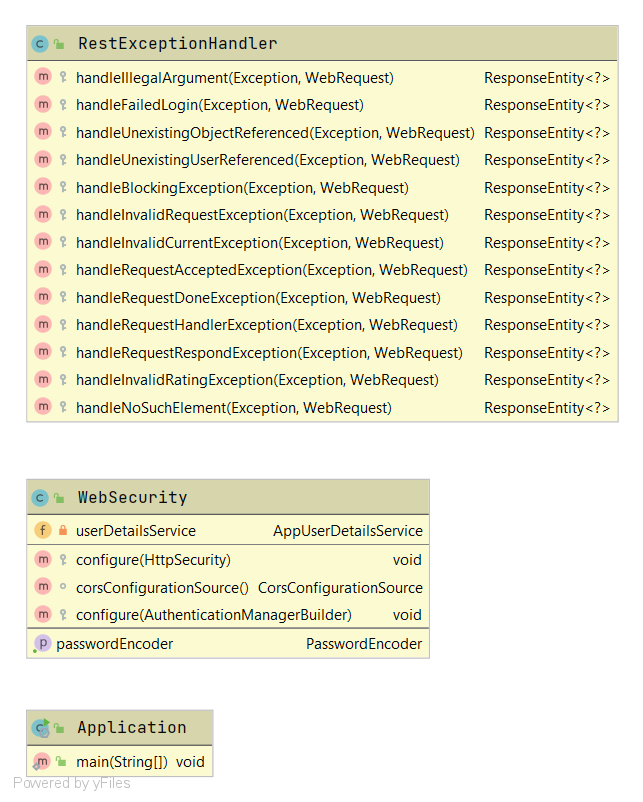
\includegraphics[scale=0.6]{slike/cs1.png} %veličina slike u odnosu na originalnu datoteku i pozicija slike
					\centering
					\caption{Struktura aplikacije i konfiguracija}
					
				\end{figure}
			
				\newpage
				
				Glavni preduvjet za obavljanje bilo kakve aktivnosti unutar aplikacije je da korisnik ima izrađen korisnički račun i prijavljen je u sustav. Klasom \textit{RegistrationDTO} modeliraju se podaci koje korisnik unosi prilikom registracije. Podaci takvog objekta služe kao predložak za stvaranje korisničkog računa. Za prijavu u sustav, provjeru korisničkog imena i lozinke te dodjeljivanje uloga zadužena je klasa \textit{AppUserDetailsService}. Korisniku može biti dodjeljena uloga ROLE\_USER i ROLE\_ADMIN kojima su određene ovlasti 
				slanja zahtjeva na kontrolere.
				
				
				\begin{figure}[H]
					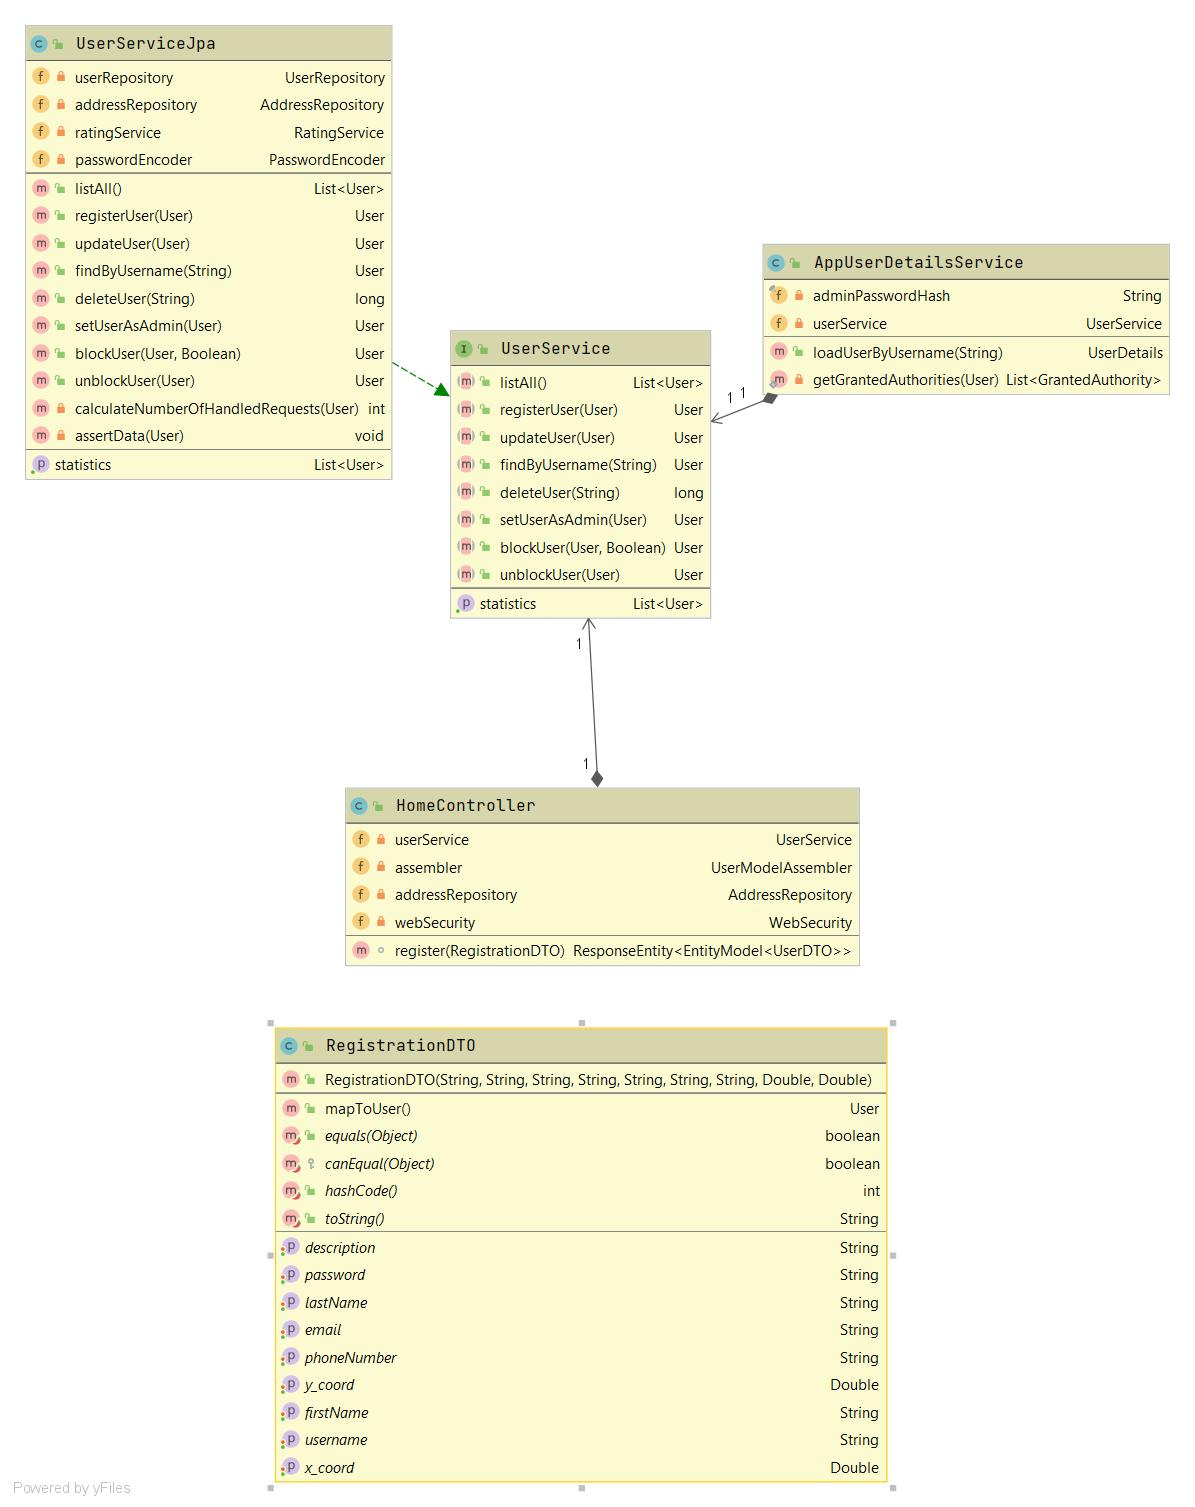
\includegraphics[scale=0.45]{slike/cs4.jpg} %veličina slike u odnosu na originalnu datoteku i pozicija slike
					\centering
					\caption{Klase koje reguliraju registraciju i prijavu}
					
				\end{figure}
			
				\newpage
				
				Slika 4.5 sadržava klase koje su ključne za aktivnosti i rad s korisnicima.
				Klasa \textit{User} predstavlja sam entitet kojim je opisan pojedini korisnik. Sadržava sve relevantne atribute za opis korisnika, konstruktore te funkciju \textit{mapToUserDTO} kojom se objekt \textit{User} pretvara u objekt pogodniji za komunikaciju sa \textit{frontendom}. \textit{UserDTO} predstavlja glavni model komunikacije s vanjskim korisnikom te skriva informacije o pojedinom \textit{Useru} koje nisu relevantne za prikaz na \textit{frontendu}.
				Omogućena je i pretvorba u suprotnom smjeru, iz klase \textit{UserDTO} u klasu \textit{User}. Klasa \textit{UserModelAssembler} omata klasu \textit{UserDTO} u oblik najprikladniji za interaktivnost prikaza, uključujući dodatne linkove. 
				Pristup i manipulacija zapisima korisnika u bazi podataka ostvaren je klasom \textit{UserRepository} koja sadrži sve standardne metode za rad sa zapisima.
				Poslovna logika koja se tiče korisnika ostvarena je u klasi \textit{UserServiceJpa}.
				\textit{UserController} zadužen je za obrađivanje zahtjeva. On inicijalizira komunikaciju sa servisom i bazom podataka i oblikuje podatke o korisnicima u odgovor na zahtjev.
				
				
			
				\begin{figure}[H]
				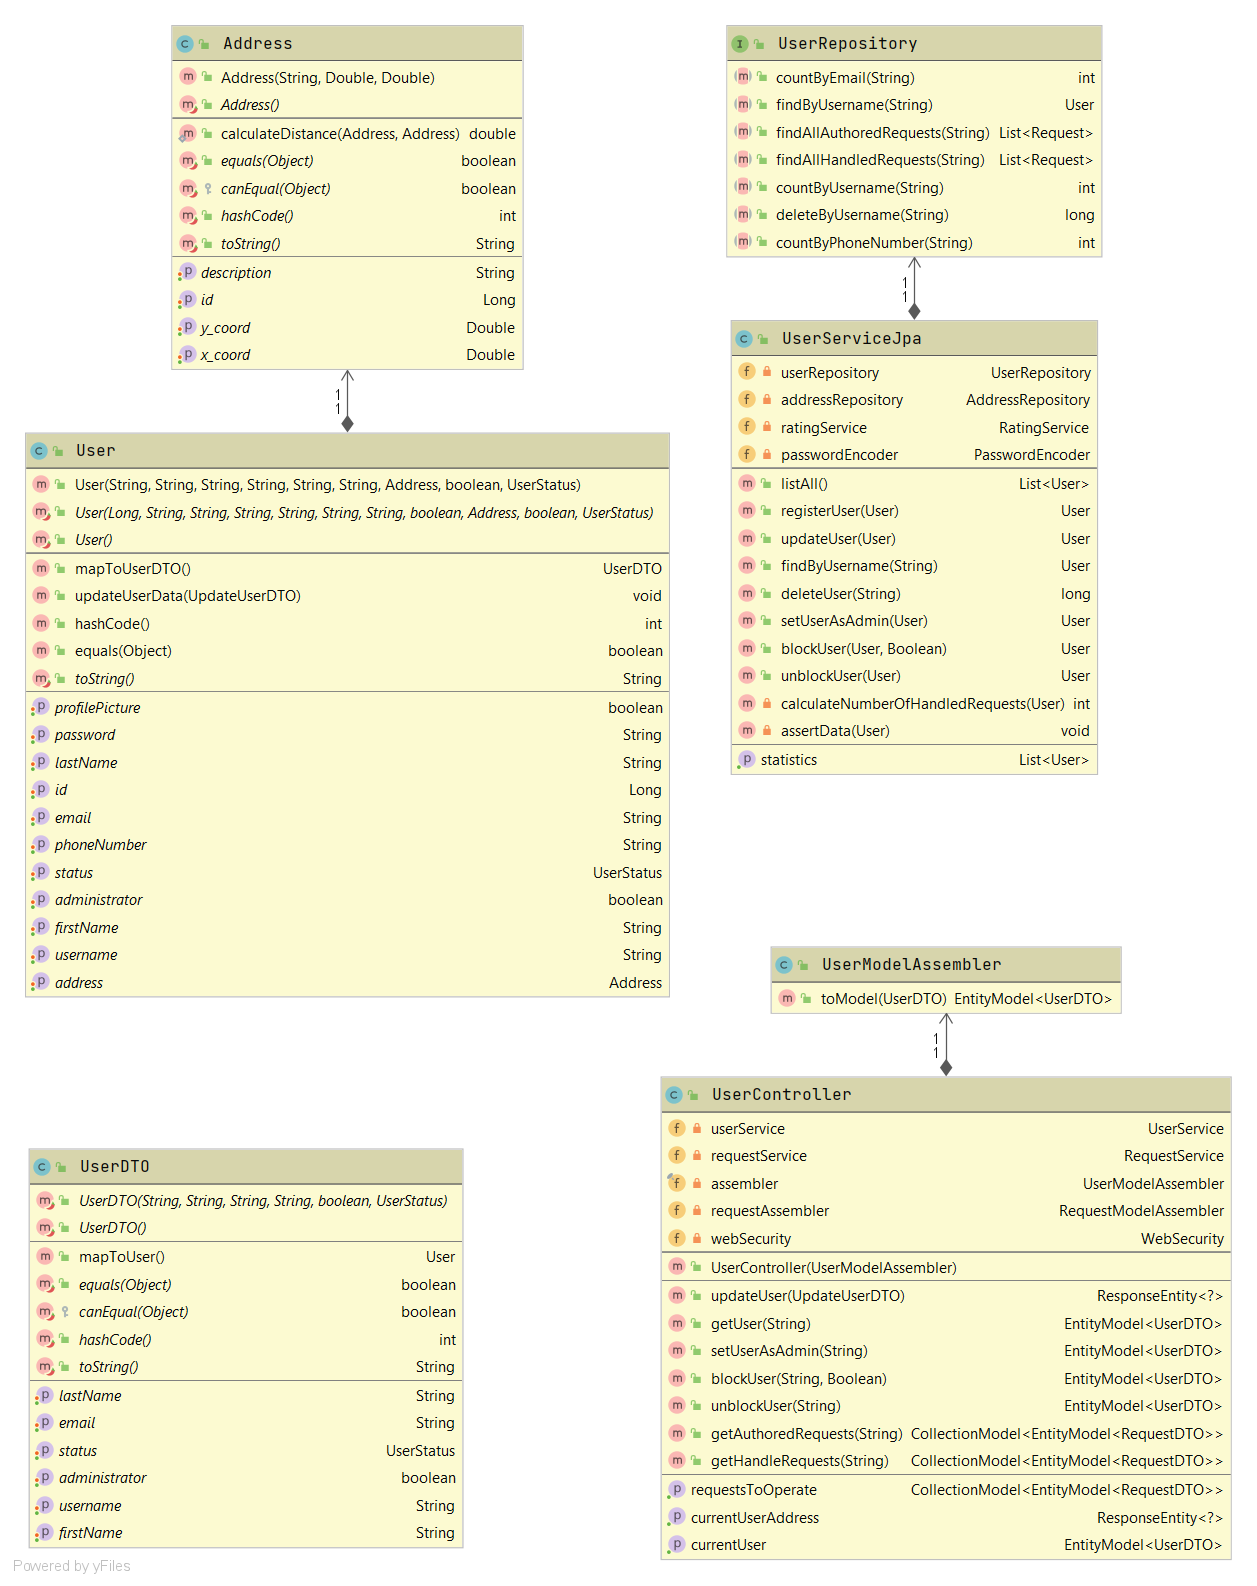
\includegraphics[scale=0.38]{slike/cs2.png} %veličina slike u odnosu na originalnu datoteku i pozicija slike
				\centering
				\caption{Klase koje reguliraju rad s korisnicima sustava}
				
				\end{figure}
			
				\newpage
				
				Klasa \textit{Request} modelira zahtjeve korisnika. Kao i u slučaju sa klasom \textit{User}, ova klasa ima pripadajuću klasu DTO-a, repozitorija, servisa i kontrolera. 
				Prilikom zadavanja zahtjeva, na kontoroler dolazi zahtjev koji u tijelu sadržava objekt tipa \textit{CreateRequestDTO} koji sadrži isključivo podatke koje unosi sam korisnik. Taj objekt je potrebno stvoriti objekt tipa \textit{Request} koristeći dobivene podatke i predefinirane podatke koji opisuju stanje zahtjeva kako bi se on mogao spremiti u bazu podataka.
				
				
			
				\begin{figure}[H]
					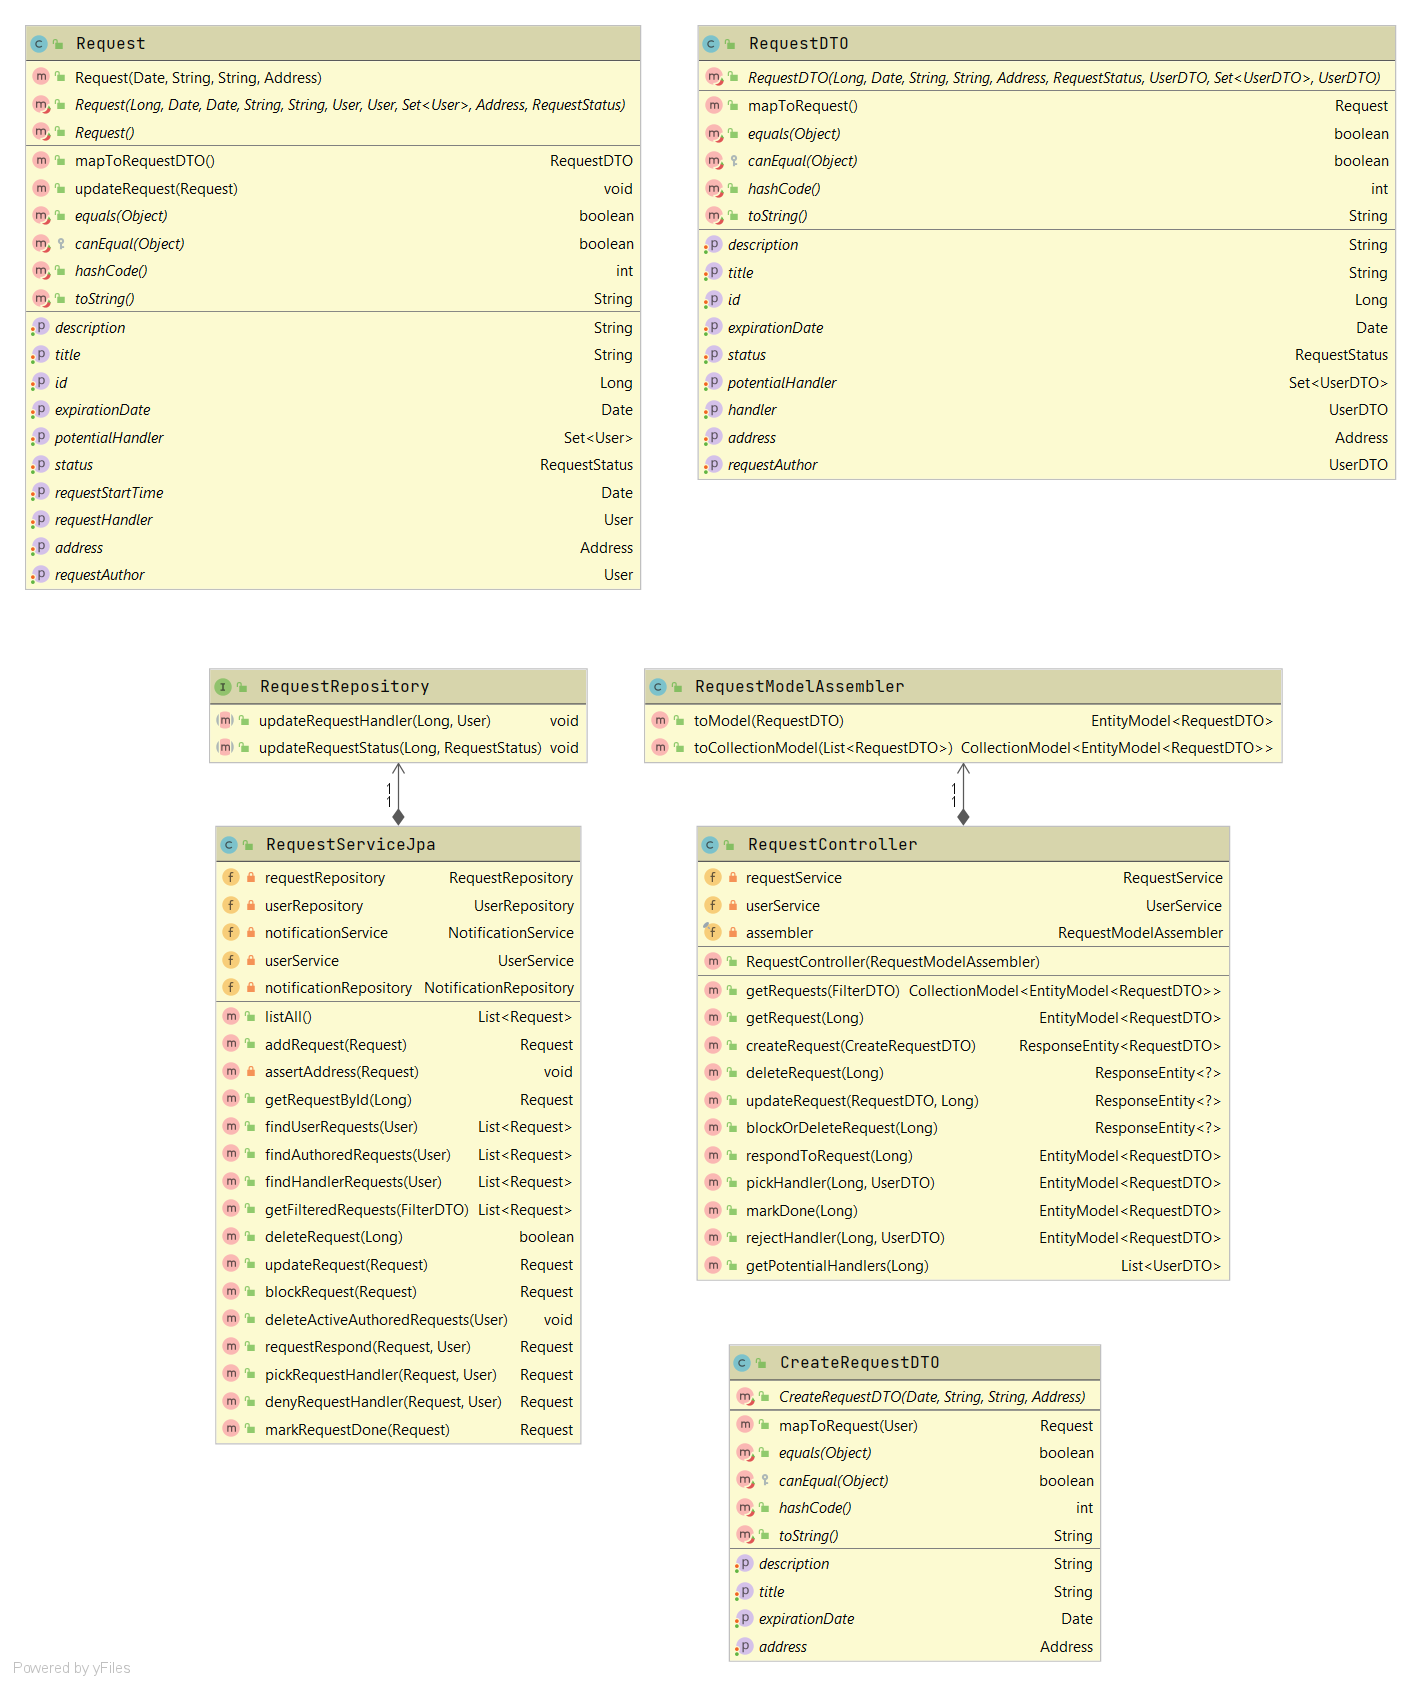
\includegraphics[scale=0.38]{slike/cs3.png} %veličina slike u odnosu na originalnu datoteku i pozicija slike
					\centering
					\caption{Klase koje reguliraju rad sa zahtjevima}
					
				\end{figure}
			
				\newpage
				
				Korisnicima je omogućeno međusobno ocjenjivanje te su na slici 4.7 prikazane klase koje služe modeliranju ocjena i ocjenjivanja. Svaka instancla klase \textit{RatingDTO} ima postavljenog korisnika koji je ocijenio te korisnika koji je ocjenjen,ocjenu, komentar te opcionalno zahtjev na koji se odnosi.
				\textit{RatingServiceJpa} omogućuje prikaz ocjena koje je pojedini korisnik autorirao te ocjena koje je pojedini korisnik dobio.			
				\begin{figure}[H]
					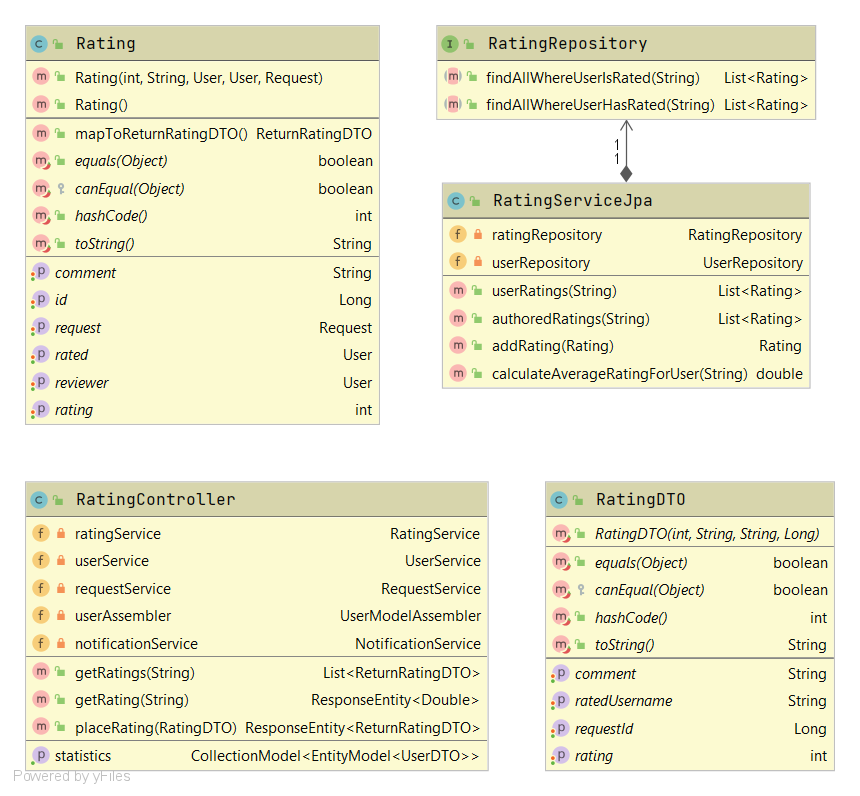
\includegraphics[scale=0.6]{slike/cs5.png} %veličina slike u odnosu na originalnu datoteku i pozicija slike
					\centering
					\caption{Klase koje reguliraju ocjenjivanje korisnika}
					
				\end{figure}
				
				
			
				
			
			
				
		
			
			
			\eject
			
		\section{Dijagram stanja}


			Dijagram stanja je tip dijagrama koji služi za opis ponašanja sustava pomoću stanja u koja se može preći nekim događajem. Na slici 4.8 prikazan je dijagram stanja jednog korisnika(koji nije administrator).Nakon prijave(ili registracije ako korisnik nema korisnički račun), korisnik odlazi na početnu stranicu aplikacije. Na početnoj stranici korisnik može: pregledati vlastiti profil, pregledati vlastite zahtjeve, pregledati profile i zahtjeve drugih korisnika, te pregledati statistiku. Klikom na "Pregled profila" korisniku se otvara vlastiti profil, te ga može izbrisati ili izmijeniti. Klikom na "Moji zahtjevi" korisnik može pregledati vlastite zahtjeve. Uz to može stvoriti novi zahtjev, blokirati postojeći, pregledati potencijalne izvršitelje nekog zahtjeva(i time prihvatiti ili odbiti nekog od potencijalnih izvršitelja) i na kraju postaviti zahtjev kao izvršen(i ocijeniti izvršitelja zahtjeva).
			Klikom na "Zahtjevi" korisniku se omogućuje pregled zahtjeva drugih korisnika i samim time se omogućava javljanje za zahtjeve. Klikom na "Profil" korisniku se otvara profil korisnika kojeg želi pregledati, te može vidjeti cjelokupnu ocjenu tog korisnika i sam ga može ocijeniti. Na kraju korisnik može pregledati i statistiku klikom na "Statistika" gdje se prikazuju 3 najbolje ocijenjena korisnika. 
			
			\begin{figure}[h]
				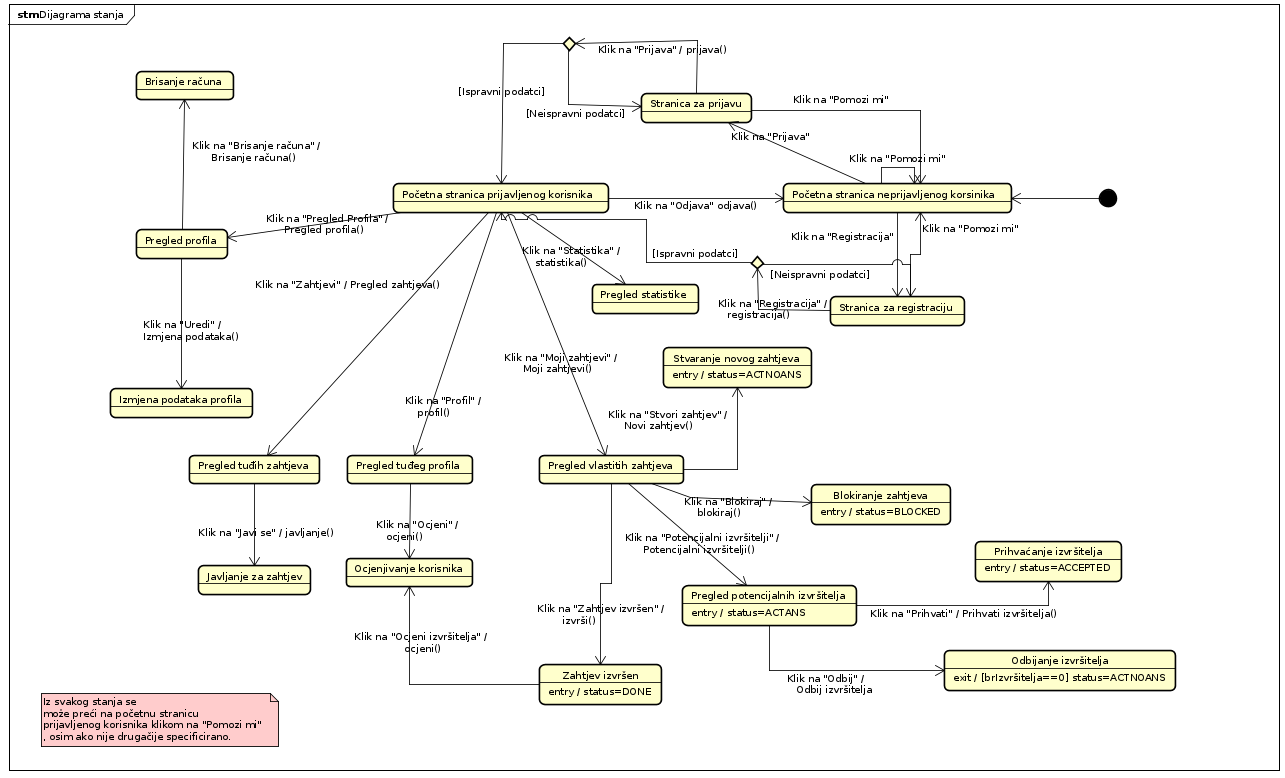
\includegraphics[height=0.47\textheight]{DijagramStanja}
				\caption{Dijagram stanja}
			\end{figure}
			
			
			\eject 
		
		\section{Dijagram aktivnosti}
			
			Slika 4.8 prikazuje aktivnost korisnika izvršitelja (ubuduće korisnik) pri javljanju na jedan aktivni zahtjev. Na početku aktivnosti korisnik pregledava aktivne zahtjeve i nije autor tih zahtjeva. Nakon toga zadaje radijus koji će se koristiti za prikaz samo onih zahtjeva koji su unutar tog radijusa u odnosu na korisnikovu lokaciju. Ukoliko nema takvih zahtjeva, korisniku se prikaže poruka da nema aktivnih zahtjeva i aktivnost se završava. Ukoliko ima takvih zahtjeva oni se prikazuju korisniku, te se čeka njegov odabir. Ukoliko korisnik ne želi odabrati zahtjev, akcija se tu završava. Ukoliko korisnik odabere neki od tih zahtjeva, korisnik će biti evidentiran kao potencijalni izvršitelj.
		
			
			\begin{figure}[H]
				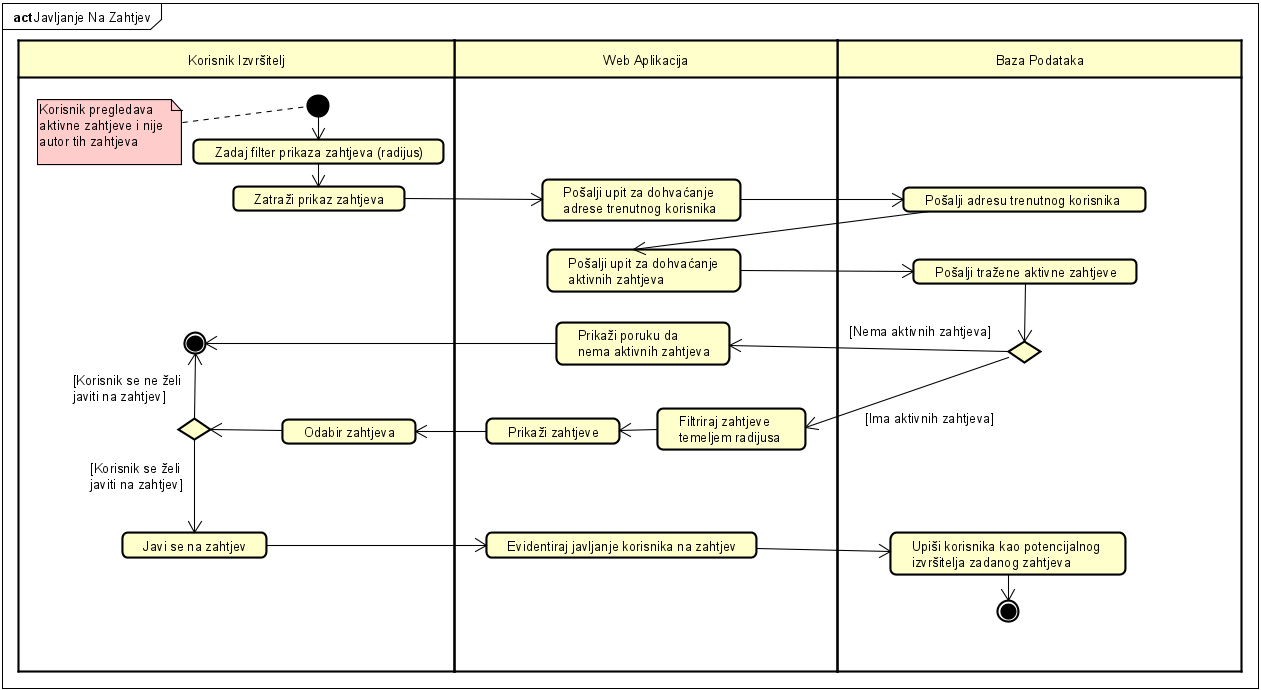
\includegraphics[scale=0.5]{slike/dijagram_aktivnosti.png} %veličina slike u odnosu na originalnu datoteku i pozicija slike
				\centering
				\caption{Aktivnost javljanja na zahtjev}
				
			\end{figure}
			
			\eject
		\section{Dijagram komponenti}
		
			Pomoću dijagrama komponenti prikazanog na slici 4.9 prikazan je međuodnos glavnih komponenti sustava.
			Najgrublja podjela komponenata koje međusobno komuniciraju u \textit{ModelViewController} (MVC) obrascu je na:
			\begin{itemize}
				\item Model koji predstavlja skup svih entiteta koji se spremaju u bazi te se nad njima vrše operacije.
				\item View kojeg predstavlja komponenta Frontend web aplikacija.
				\item Controller koji služi za primanje HTTP zahtjeva i slanje odgovora.
			\end{itemize}
			
			Frontend web aplikacija komunicira sa ostatkom aplikacije pri posluživanju statičkog sadržaja poput HTML, CSS i JS datoteka te sa backend dijelom aplikacije u formatu JSON.
			Posluživanje sadržaja frontend dijelu aplikacije ovisi o ulozi korisnika kojemu se poslužuje te
			shodno ulozi komponenta Router odlučuje o tome koje se datoteke poslužuju. Također, u to su uključene i datoteke JavaScript libraryja React koji se koristi u oblikovanju korisničkog sučelja.
			
			Format JSON glavni je format za komunikaciju sa REST API-jem kojeg aplikacija koristi.
			REST API po primitku JSON objekta mapira ga u pripadajući objekt u Javi. Vrijedi i obrnuto, prilikom slanja Java objekta on se prethodno pretvara u pripadajući JSON i u tom obliku šalje HTTP protokolom.
			
			
			Komponenta kontrolera putem DTO objekata ostvaruje komunikaciju sa REST API-jem i poslovnom logikom aplikacije.
			Pristup bazi na backendu nudi se sučeljem s komponentom \textit{JPARepositories} 
			te ona služi kao glavna komunikacija aplikacije i SQL baze podataka u jeziku JPQL.
			
			 \begin{figure}[h]
			 	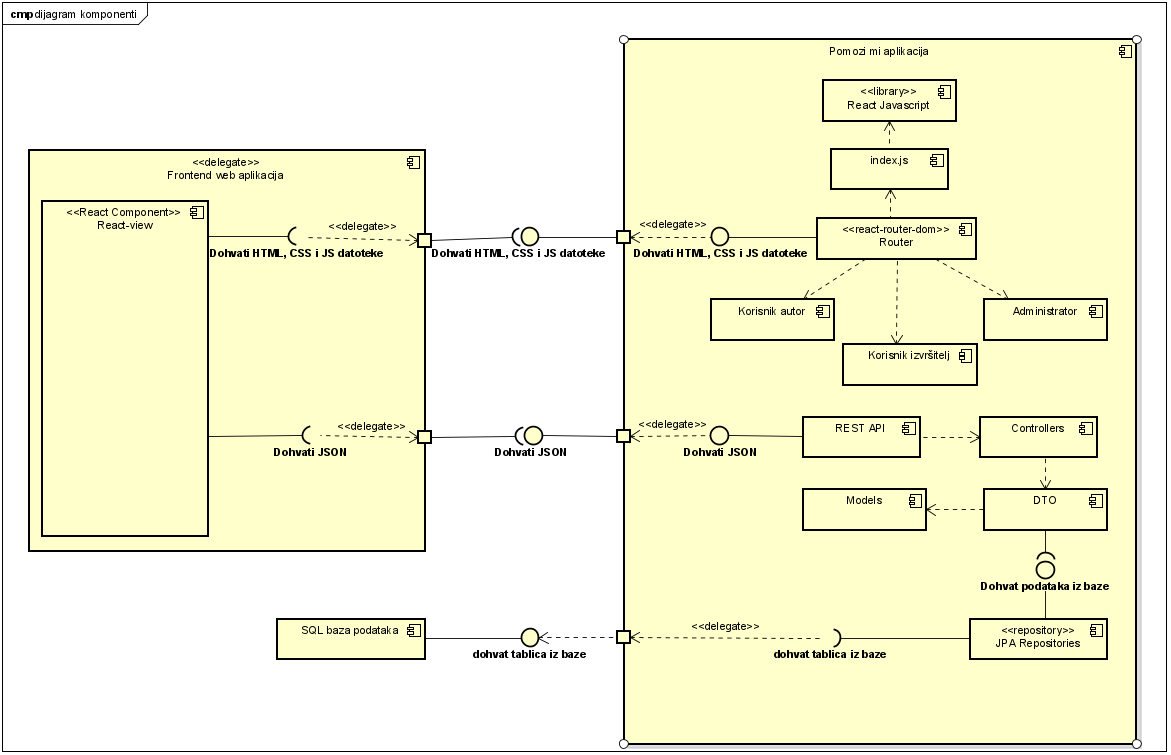
\includegraphics[height=0.5\textheight]{dijagramKomponenti}
			 	\caption{Dijagram komponenti}
			 \end{figure} 
			
	
	
\chapter{Implementacija i korisničko sučelje}
		
		
		\section{Korištene tehnologije i alati}

		Komunikacija našem u timu je realizirana korištenjem aplikacija Discord\footnote{https://discord.com/} i WhatsApp\footnote{https://www.whatsapp.com/}.\\ Za izradu UML dijagrama korišten je alat Astah Professional\footnote{http://astah.net/editions/professional}, a kao sustav za upravljanje
izvornim kodom Git\footnote{https://git-scm.com/}. Udaljeni repozitorij projekta je dostupan na web platformi GitLab\footnote{https://gitlab.com/}, a kao razvojno okruženje korišten je IntelliJ IDEA\footnote{https://www.jetbrains.com/idea/} - tvrtke JetBrains\footnote{https://www.jetbrains.com/} te Microsoftov Visual Studio Code\footnote{https://visualstudio.microsoft.com/
}. 
	\\
	 Naša aplikacija napisana je koristeći Spring Framework\footnote{https://spring.io/} i jezik Java\footnote{https://www.oracle.com/java/} za izradu backenda te React\footnote{https://reactjs.org/} - JavaScript library za izradu frontenda. React je open-source, front end, JavaScript knjižnica za izgradnju korisničkog sučelja ili UI komponenti. Održavaju ga Facebook i zajednica pojedinačnih programera i tvrtki. Spring razvojno okruženje je Java platforma koja pruža široki panel opcija kao podrški
razvoju Java aplikacija. Spring rukuje infrastrukturom, tako da programer može usmjeriti svoj
fokus na razvoj aplikacije. \\
Tijekom izrađivanja aplikacije koristili smo i Postman\footnote{https://www.postman.com/} za simuliranje HTTP zahtjeva nad aplikacijom, Google Drive\footnote{https://workspace.google.com/products/drive/} za efikasno dijeljenje organizacijskih informacija i raznih datoteka. 
Baza podataka se nalazi na poslužitelju u oblaku Amazon
Web Services\footnote{https://aws.amazon.com/}.			
			
			\eject 
		
	
		\section{Ispitivanje programskog rješenja}

	
			
			\subsection{Ispitivanje komponenti}

			\textbf{Unit testovi za Service sloj}
			\bigskip
			\newline
			Za izradu unit testova korišten je framework Mockito, koji simulira rad objekata koje testni razred koristi.  
			 @Mock anotacija stvara objekt koji se koristi u testiranju, on ne izvodi svoje normalne metode, već samo simulira njihov rad.
			\bigskip
			\bigskip
			
			\bigskip
			\textbf{UserServiceJpa unit test}
			\bigskip
			
			\textit{listAll()} - U unit testu stvaramo 3 nova korisnika i simuliramo metodu listAll(). Očekivani rezultat je lista tri korisnika. Zatim pozovemo metodu listAll() i provjerimo vraća li ta metoda ispravni izlaz.
			
			\textit{registerUser()} - Unit testovi za ovu metodu ispituju ponašanje sustava za neuspješnu i uspješnu registraciju.
			
			\textit{updateUser()} - Testovi ispituju ponašanje sustava prilikom pokušaja ažuriranja korisničkih podataka. Pokriveni su slučajevi potpunih i nepotpunih podataka za ažuriranje.
			
			\textit{findByUsername()} - Testovi ispituju ponašanje sustava pri pretraživanju korisnika za postojeće i nepostojeće korisničko ime.
			
			\textit{getStatistics()} - Ukoliko ne postoje registrirani korisnici pri pozivu ove metode, ona bi trebala vratiti praznu listu. Ako postoje registrirani korisnici, ali ne njih više od dva, metoda bi trebala vratiti samo listu od tog jednog ili dva korisnika, tako da je prvi onaj bolje ocjenjeni. Ako postoji tri ili više registriranih korisnika metoda bi trebala vratiti listu od tri najbolje ocjenjena korisnika. Testira se i u kojem poretku je metoda vratila najbolje ocijenjene korisnike.
			
			\bigskip
			\bigskip
			\textbf{RatingServiceJpa unit test}
			\bigskip
			
			\textit{calculateAverageRatingForUser()} - Metoda ispituje  izračun prosječne ocjene za korisnika. Ulaz je korisničko ime, a izlaz ovisi o postojanju korisnika s danim korisničkim imenom i postojanju ocjena.
			
			\bigskip
			\bigskip
			\textbf{RequestServiceJpa unit test}
			\bigskip
			
			\textit{addRequest()} - Metoda testira potpunost podataka prilikom stvaranja zahtjeva. Ako je predan zahtjev koji je potpun i točan metoda bi trebala uspješno dodati zahtjev. U suprotnom metoda testira odgovarajuće iznimke.
			
			\bigskip
			\begin{figure}[H]
				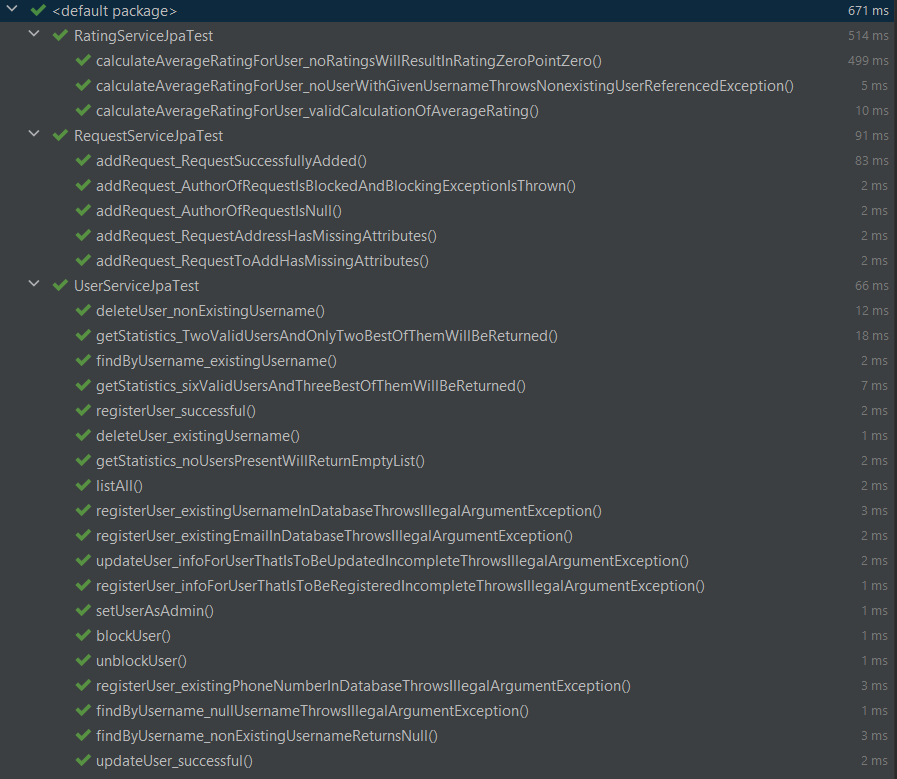
\includegraphics[scale=0.8]{slike/unit_testovi.png}
				\centering
				\caption{Rezultati unit testova}
				
			\end{figure}
			
			
			\subsection{Ispitivanje sustava}
			
			Za ispitivanje sustava korišten je alat za automatizirano testiranje Selenium WebDriver. Ispitni slučajevi pisani
			su u jeziku Java. \newline
			
			Cilj ispitivanja sustava je ispitati ponašanje sustava u cjelini, onako kako ga vidi 
			korisnik aplikacije te dostupnost svih funkcionalnosti koje korisnik može koristiti.
			Napisani ispitni slučajevi prije svega su ispitivali pravilan izgled komponenti i funkcionalnosti koje se nude kroz korisničko sučelje u ovisnosti o stanju sustava, stanju pojedinog zahtjeva i ovlastima korisnika.
			Testiranje je koristilo dva korisnika već registrirana u sustav, jednog s ovlastima običnog korisnika i drugog s ovlastima administratora.\newline 
			
			Komponente koje najviše ovise o ovlastima i stanju sustava su komponenta za prikaz pojedinog zahtjeva i komponenta profila korisnika.
			Za primjer, funkcionalnosti rada sa zahtjevima testiraju metode:
			\begin{packed_enum}
				
				\item \textit{createRequestExpectedBehaviour()} - očekivani unos u formu zahtjeva
				\item \textit{createRequestNoTitle()} - neispravan unos u formu zahtjeva
				\item \textit{viewNonAuthoredRequest()} - prisutnost komponenti za javljanje na zahtjev
				\item \textit{viewAuthoredRequest()} - prisutnost komponenti za blokiranje zahtjeva
				\item \textit{viewAuthoredRequestWithPotentialHandlers()} - prisutnost komponenti za pregled potencijalnih izvršitelja 
			\end{packed_enum}
			
		
			
			Testni slučajevi fokusirali su se na različite situacije i rubne slučajeve u prikazu i funkcionalnostima.
			Rubni slučajevi poput pogrešnog unosa u formu ili nedostatka nekog unosa se u aplikaciji signaliziraju različitim porukama o pogrešci. 
			Testne metode za takve slučajeve prije svega su se fokusirali na traženje odgovarajuće poruke o pogrešci.
			Konkretan primjer za to su testni slučajevi unosa pogrešnih korisničkih podataka u formu za prijavu. \newline 
			
			Neimplementirana funkcionalnost koja je također testirana je traka za pretraživanje. 
			Testom je pokazano da akcijama nad njom se ne mjenja stanje sustava i ne remeti se normalan tijek funkcioniranja aplikacije. \newline
			
			Glavnu prepreku za automatizaciju ispitivanja sustava predstavljala je priroda testiranog sustava. 
			Sustav se sastoji od brojnih aktivnosti koje se mogu izvoditi samo jednom, poput javljanja na pojedini zahtjev ili 
			biranja izvršitelja za zahtjev te aktivnosti koje zahtijevaju slijednu interakciju više korisnika.
			Takve akcije teško je automatizirano ispitivati zato što to neminovno u sustavu akumulira velik broj zahtjeva samo za testiranje 
			ili testove nije moguće ponavljati više puta, čime se u potpunosti gubi njihova svrha.
			Stoga su navedene funkcionalnosti izostavljene iz automatiziranog ispitvanja alatom Selenium i odrađene ručno.
			
			
			
			
			\begin{figure}[H]
				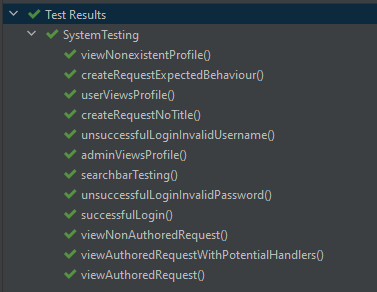
\includegraphics[scale=1.2]{slike/selenium-testing.png}
				\centering
				\caption{Rezultati testova sustava}
				
			\end{figure}
			
			 
			
			\eject 
		
		
		\section{Dijagram razmještaja}
			
			Na slici 5.3 nalazi se dijagram razmještaja koji prikazuje raspored programske podrške aplikaciji unutar sklopovlja.
			
			Sa strane korisnika aplikacije, sklopovlje predstavlja njegovo računalo, mobilni telefon ili bilo koji drugi uređaj s pristupom internetu i instaliranim browserom.
			Internetski browser zadužen je za uspostavu konekcije sa poslužiteljem koja će omogućiti slanje i posluživanje zahtjeva.
			Sa strane poslužitelja sklopovlje predstavlja serversko računalo.
			Dvije glavne usluge koje se nalaze na serverskom računalu su baza podataka i web server koje su nužne za posluživanje zahtjeva.
			
			Komunikacija između korisnika i poslužitelja vrši se putem \textit{stateless} HTTP protokola. 
			Tijekom slanja zahtjeva serveru, korisnikov browser ima otvorenu jednu HTTP vezu prema serveru.
			S druge strane server može posluživati više zahtjeva iz više različitih izvora te stoga može imati i više aktivnih HTTP veza.
			
			\begin{figure}[h]
				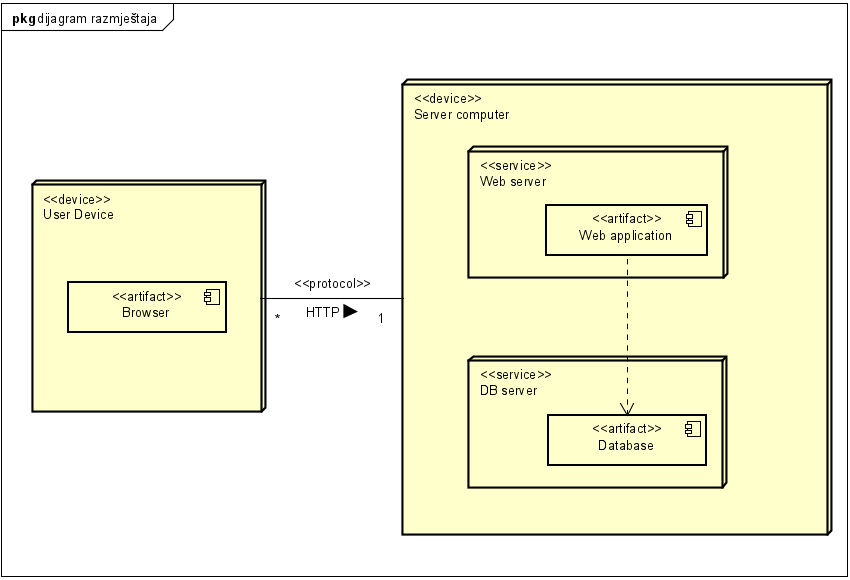
\includegraphics[height=0.44\textheight]{dijagramRazmjestaja}
				\caption{Dijagram razmještaja}
			\end{figure} 
			
			\eject 
		
		\section{Upute za puštanje u pogon}
		
			Grupa TODO odlučila je aplikaciju pustiti u pogon koristeći Amazon Web Services (AWS). Za korištenje AWS-a potrebno se registrirati i ostaviti podatke za plaćanje, ali koriste se besplatne mogućnosti dostupnih usluga te ništa neće biti naplaćeno. 
			
			Korisnik nakon registracije, odlazi na adresu \url{https://us-east-2.console.aws.amazon.com/console/home}, gdje dobiva prikaz dostupnih usluga:
			
			\begin{figure}[h]
				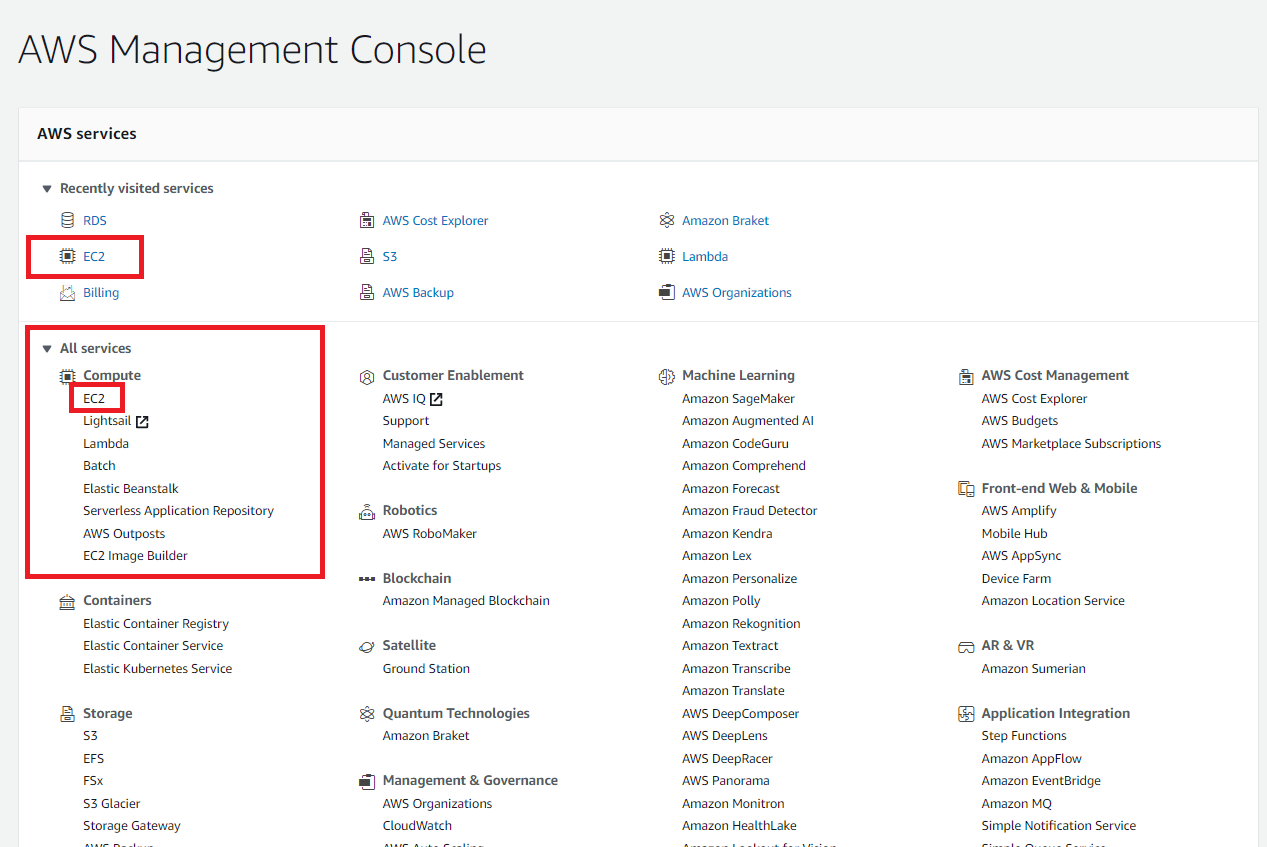
\includegraphics[scale=0.5]{slike/deployment_slike/awshome.png}
				\centering
				\caption{Dostupne AWS usluge}
				
			\end{figure}
		
			Biramo link EC2  koji nas vodi na iduću stranicu,gdje želimo stisnuti na pokretanje nove instance virtualnog stroja (Slika 5.4), potom odabiremo operacijski sustav virtualnog stroja(Slika 5.5). Biramo OS sa slike zato što je dostupan za besplatno korištenje. U idućem koraku ponovo odabiremo besplatan tip instance (Slika 5.6), klikamo Review and Launch i Launch, postavljamo i preuzimamo ključ za pristup instanci (neće biti potreban, al ga je dobro pričuvat). Posljednji put pritišćemo Launch i pokreće se instanciranje virtualnog stroja. Zatim na adresi \url{https://us-east-2.console.aws.amazon.com/ec2/v2/home} možemo pregledati vlastite instance virtualnih strojeva (Slika 5.7). Na "running" instancu desni klik i Connect. Možemo birati više načina spajanja, biramo treću opciju zbog jednostavnosti i pritišćemo gumb Connect (Slika 5.8). Otvara nam se linux terminal u browseru (Slika 5.9) i možemo krenuti s konfiguracijom virtualnog stroja.
			
			
			\noindent Prvo unosimo naredbu:
			\begin{center}
				\$ sudo yum update
			\end{center}
				kako bi primjenili ažuriranja. Za uspješno puštanje u pogon potrebni su nam Java, Git i Maven. Njih ćemo instalirati redom upisujući naredbe
				\begin{center}
					\$ sudo yum install java-11
				\end{center}
			\begin{center}
				\$ sudo yum alternatives  \texttt{--}config java
			\end{center}
			otvara nam se izbornik te odabiremo željenu verziju jave (Java 11 Amazon Corretto) unosom rednog broja pored imena verzije.
			Maven instaliravamo sljedećim nizom naredbi:
			\begin{center}
				\$ sudo wget http://repos.fedorapeople.org/repos/dchen/apache-maven/epel-apache-maven.repo -O /etc/yum.repos.d/epel-apache-maven.repo
				
				\$ sudo sed -i s/$\backslash$\$releasever/6/g /etc/yum.repos.d/epel-apache-maven.repo
				
				\$ sudo yum install -y apache-maven
			
				\$ mvn --version
			\end{center}
			Dalje, unosimo naredbe:
			\begin{center}
				\$ sudo yum install git -y
				
				\$ git clone \{adresa repozitorija\}
			\end{center}
			Nakon toga potrebno se pozicionirati u direktorij izvornog koda (onaj gdje se nalazi pom.xml), i pokrenuti instalaciju naredbom:
			\begin{center}
				\$ mvn clean install
			\end{center}
			Nakon instalacije, u direktoriju /target nalazi se .jar datoteka koja predstavlja našu izgrađenu aplikaciju. Aplikaciju pokrećemo izvođenjem sljedeće naredbe:
			\begin{center}
				\$ nohup java -jar \{ime aplikacije\}.jar
			\end{center}
			Aplikacija je nakon nekoliko trenutaka pokrenuta i moguće joj je pristupiti preko javne adrese instance, na portu 8080, ali tek nakon što u AWS konzoli podesimo parametre sigurnosti, upute za to ostavljamo da korisnik sam prouči: \url{https://docs.aws.amazon.com/AWSEC2/latest/UserGuide/ec2-security-groups.html}
		
		
		
			
			\begin{figure}[h]
				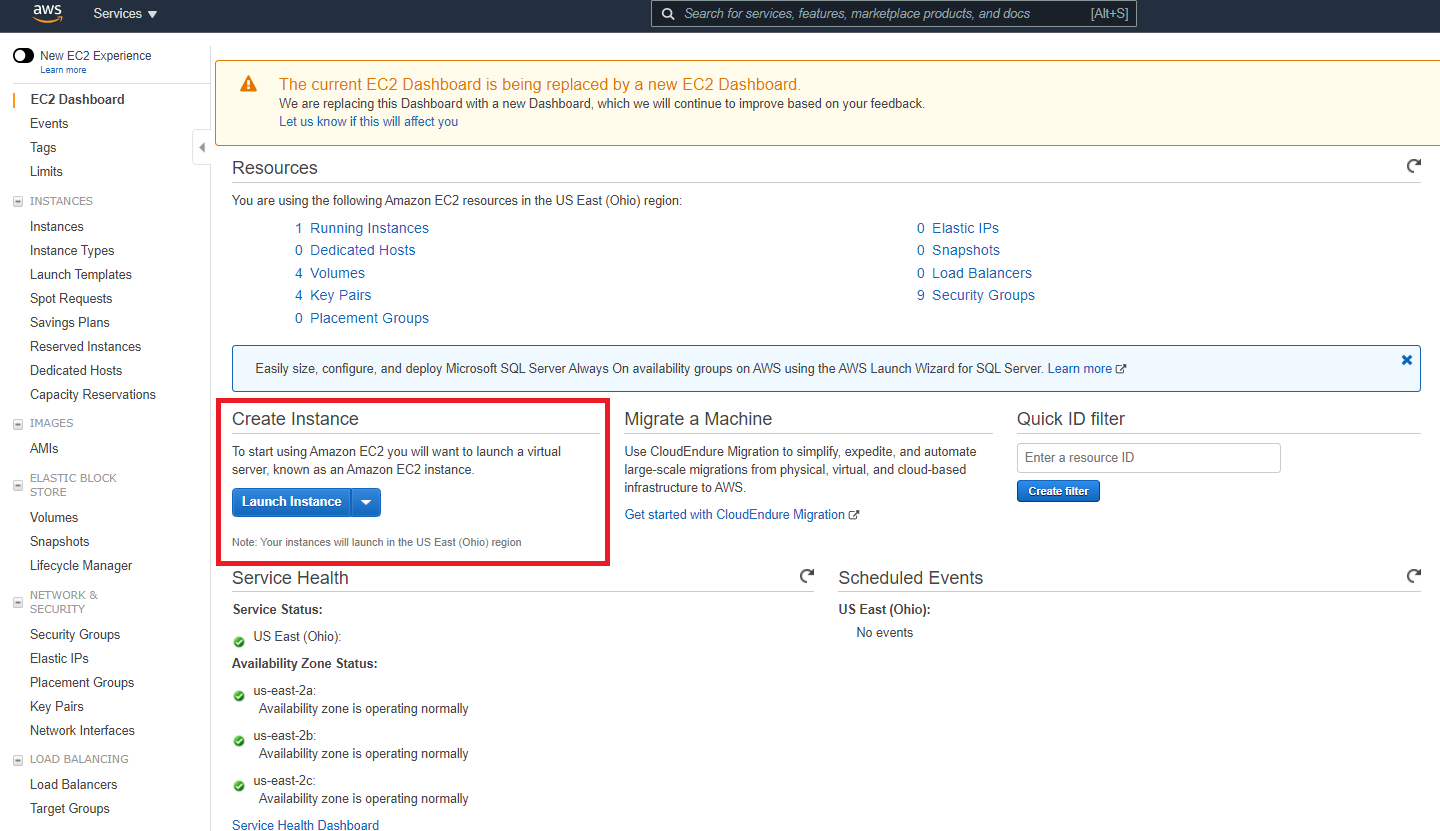
\includegraphics[width=\textwidth]{slike/deployment_slike/launchingInstance.png}
				\centering
				\caption{Pokretanje inicijalizacije}
			\end{figure}
		
			\begin{figure}[h]
				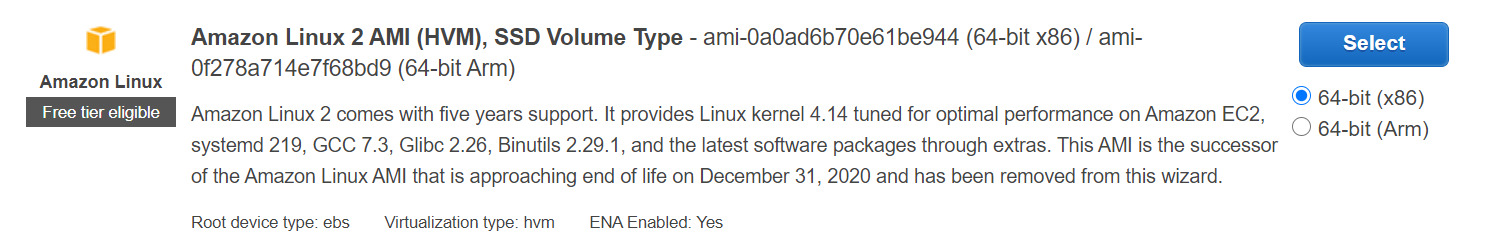
\includegraphics[width=\textwidth]{slike/deployment_slike/virtualOS.png}
				\centering
				\caption{Odabrani OS}
			\end{figure}
		
			\begin{figure}[h]
				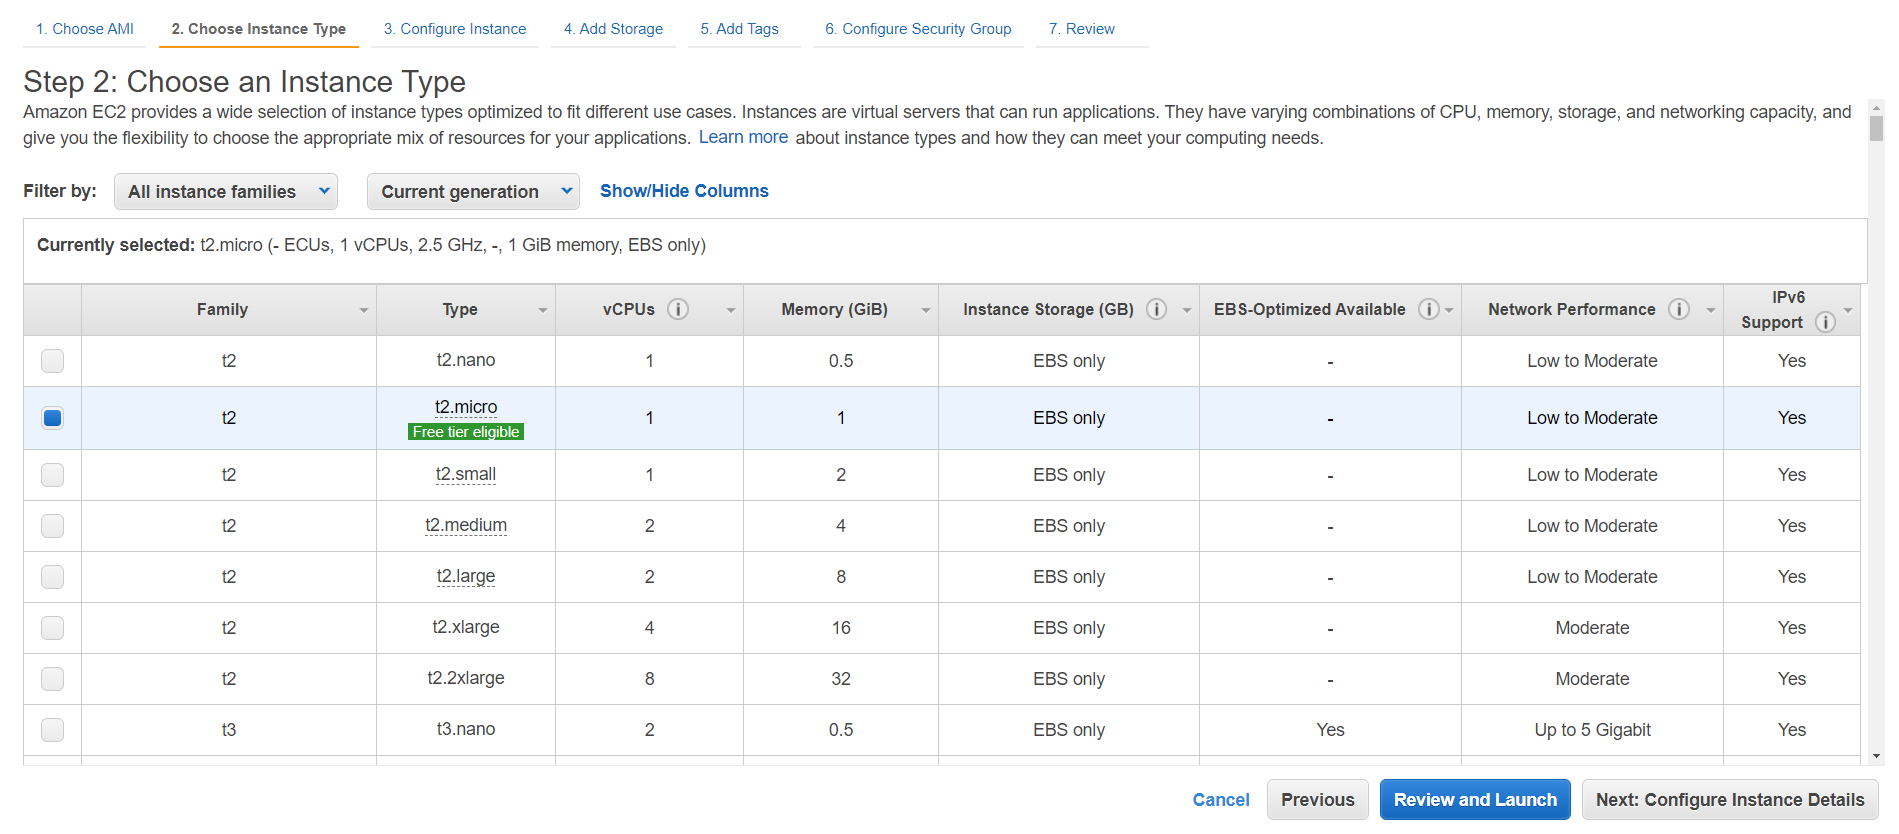
\includegraphics[width=\textwidth]{slike/deployment_slike/instanceType.png}
				\centering
				\caption{Tip instance}
			\end{figure}
			
			\begin{figure}[h]
				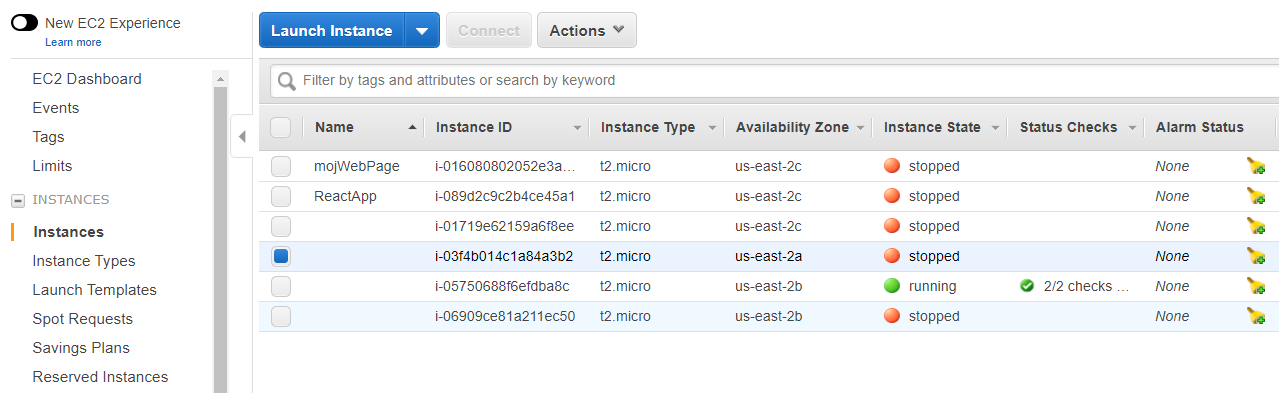
\includegraphics[width=\textwidth]{slike/deployment_slike/mojeInstance.png}
				\centering
				\caption{Instance}
			\end{figure}
			
			\begin{figure}[h]
				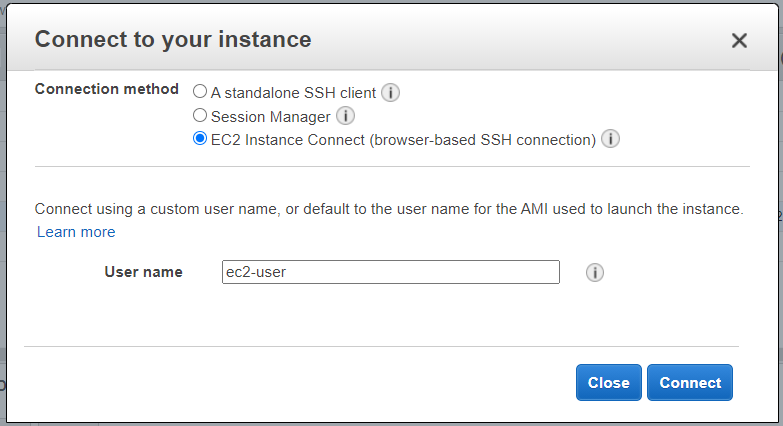
\includegraphics[width=\textwidth]{slike/deployment_slike/instanceConnect.png}
				\centering
				\caption{Spajanje na virtualni stroj}
			\end{figure}
		
			\begin{figure}[h]
				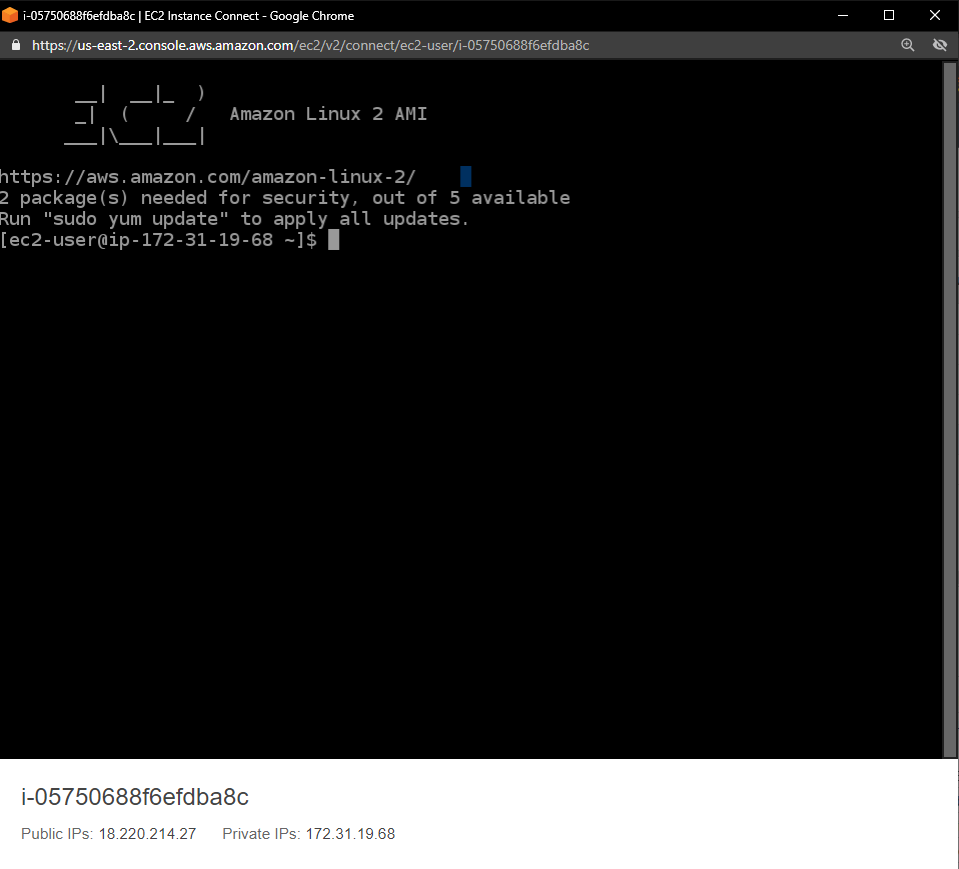
\includegraphics[width=\textwidth]{slike/deployment_slike/browserTerminal.png}
				\centering
				\caption{Browser terminal}
			\end{figure}
			
			\eject 
	\chapter{Zaključak i budući rad}
		
		\textbf{\textit{dio 2. revizije}}\\
		
		 \textit{U ovom poglavlju potrebno je napisati osvrt na vrijeme izrade projektnog zadatka, koji su tehnički izazovi prepoznati, jesu li riješeni ili kako bi mogli biti riješeni, koja su znanja stečena pri izradi projekta, koja bi znanja bila posebno potrebna za brže i kvalitetnije ostvarenje projekta i koje bi bile perspektive za nastavak rada u projektnoj grupi.}
		
		 \textit{Potrebno je točno popisati funkcionalnosti koje nisu implementirane u ostvarenoj aplikaciji.}
		 
		 \section{Izrada projekta i tehnički izazovi}
		 
		 Izrada projekta protezala se kroz period od 12 tjedana. Prvi dio izrade fokusirao se na definiranje korisničkih zahtjeva i zahtjeva sustava, dok se drugi dio okrenuo ka implementaciji definiranog sustava.
		 
		 Imajući na umu da nitko iz projektne grupe nije bio upoznat sa tehnologijama koje su se koristile (Spring Framework i React), glavni izazov predstavljalo je upoznavanje s novim tehnologijama. \newline
		 Inicijalno, to je otežavalo vremensko planiranje i nošenje sa klasičnim problemima uporabe Springa i Reacta koji se mogu zaobići korištenjem koncepta \textit{best practice}. \newline 
		 
		 \subsection{Tehnički izazovi korištenja radnog okvira Spring}
		 Najveći izazov prilikom korištenja radnog okvira Spring bili su u uspostavi autentikacije i autorizacije. Radi jednostavnost izvedbe inicijalne inačice, odlučeno je za konfiguraciju sigurnosti aplikacije koristiti već postojeću Springovu klasu \textit{WebSecurityConfigurerAdapter}. Najduže je trajalo uspostavljanje konfiguracije autentikacije putem \textit{UserDetailsSerivce}-a iz razloga nepotpunosti i manjkavosti informacija o funkcionalnostima navedenog service-a na internetu i čestih neočekivanih ponašanja koja su posljedica različitih konfiguracija sigurnosti u referentnim primjerima i našoj aplikaciji. Autentikacija je uspješno uspostavljena pregledavanjem implementacije korištenih klasa i službene dokumentacije. 
		 Manjkavost koju uviđamo u našoj izvedbi sigurnosti je nekorištenje tokena, već svaki zahtjev mora sadržavati autentikacijske podatke \textit{username} i \textit{password}.
			 
	
		
		\subsection{Izazovi korištenja knjižnice React}
		Glavnina tehničkih izazova korištenja knjižnice React je proizašla iz potrebe za adaptacijom komponenti koje React nudi. Kao kompromis između pisanja vlastitih i relativno teške adaptacije već postojećih komponenti, glavni \textit{layout} web stranice izrađen je ručno i uz pomoć \textit{Bootstrapa}, dok su se za pojedine komponente unutar stranice koristile komponente \textit{Semantic-UI}.
		
		
		 \eject
		 \section{Budući rad}
		 S obzirom na kratko vrijeme za izvedbu aplikacije i ograničeno prethodno iskustvo projektnog tima, prva inačica aplikacije ostaje otvorena za neka poboljšanja. U ovom odjeljku opisani su prijedlozi za restrukturiranje dijela funkcionalnosti te koje dodatne funkcionalnosti bi poboljšale aplikaciju.\newline 
		 
		 Restrukturiranje sigurnosti i izmjene potrebne za uvođenje \textit{JWT tokena} kao sredstva autentikacije prva je i najbitnija potrebna izmjena. Time se osigurava veća sigurnost podataka u odnosu na slanje \textit{passworda} u svakom HTTP zahtjevu. Dodatno, e-mail verifikacijom unesene adrese prilikom registracije potrebno je osigurati da se nitko osim stvarnog posjednika adrese ne može registrirati u sustav. \newline
		  
		 
		 Kako bi se osigurala kvalitetnija komunikacija i interakcija između korisnika aplikacije te bolji \textit{user experience} dodatne implementacija funkcionalnosti pretraživanja korisnika i zahtjeva te \textit{chat} koje nisu izvedene u prvoj inačici je nužna. \newline
		 
		 Od zahtjevanih i predviđenih funkcionalnosti aplikacije u prvoj inačici nisu implementirane:
		 \begin{packed_enum}
		 	
		 	\item Brisanje korisničkog računa
		 	\item Prikaz lanaca povjerenja

		\end{packed_enum}		
		Predviđene i neimplementirane funkcionalnosti bit će ukljućene u iduću inačicu aplikacije. 	
		 
		 \eject
		 
		 \section{Zaključak}
		 Izvođenje ovog projekta uvelike je pridonjelo praktičnom iskustvu svih članova projektne grupe. Nadasve najbitnije znanje koje je projektna grupa dobila je uvid u cjelokupni proces razvoja određenog programskog proizvoda, počevši sa planiranjem, razradom pa sve do \textit{deployment}-a. To znanje je učinilo dosadašnja znanja članova projektne grupe kompletnijima i primjenjivijima. Također, projekt je potaknuo grupu na aktivnije korištenje već gotovih knjižnica i komponenata i njihovu adaptaciju za specifične potrebe projekta.
		 \eject
		 
		 
		
		\eject 
	\chapter*{Popis literature}
		\addcontentsline{toc}{chapter}{Popis literature}
	 	
 		\textbf{\textit{Kontinuirano osvježavanje}}
	
		\textit{Popisati sve reference i literaturu koja je pomogla pri ostvarivanju projekta.}
		
		
		\begin{enumerate}
			
			
			\item  Programsko inženjerstvo, FER ZEMRIS, \url{http://www.fer.hr/predmet/proinz}
			
			\item  I. Sommerville, "Software engineering", 8th ed, Addison Wesley, 2007.
			
			\item  T.C.Lethbridge, R.Langaniere, "Object-Oriented Software Engineering", 2nd ed. McGraw-Hill, 2005.
			
			\item  I. Marsic, Software engineering book``, Department of Electrical and Computer Engineering, Rutgers University, \url{http://www.ece.rutgers.edu/~marsic/books/SE}
			
			\item  The Unified Modeling Language, \url{https://www.uml-diagrams.org/}
			
			\item  Astah Community, \url{http://astah.net/editions/uml-new}
		\end{enumerate}
		
		 
	
	
	\begingroup
	\renewcommand*\listfigurename{Indeks slika i dijagrama}
	%\renewcommand*\listtablename{Indeks tablica}
	%\let\clearpage\relax
	\listoffigures
	%\vspace{10mm}
	%\listoftables
	\endgroup
	\addcontentsline{toc}{chapter}{Indeks slika i dijagrama}


	
	\eject 
		
	\chapter*{Dodatak: Prikaz aktivnosti grupe}
		\addcontentsline{toc}{chapter}{Dodatak: Prikaz aktivnosti grupe}
		
		\section*{Dnevnik sastajanja}
		
	
				
		\begin{packed_enum}
			\item  sastanak
			
			\item[] \begin{packed_item}
				\item Datum: 4. listopada 2020.
				\item Prisustvovali: H.Rom, Ž.Rački, M.Stanić, D.Oreč, D.Milde, A.Ilinović, M.Bakšić
				\item Teme sastanka:
				\begin{packed_item}
					\item  upoznavanje
					\item  dogovor o tehnologijama za projekt
					\item  dogovor oko uloga
				\end{packed_item}
			\end{packed_item}
			
			\item  sastanak 
			\item[] \begin{packed_item}
				\item Datum: 13. listopada 2020.
				\item Prisustvovali: H.Rom, Ž.Rački, M.Stanić, D.Oreč, D.Milde, A.Ilinović, M.Bakšić
				\item Teme sastanka:
				\begin{packed_item}
					\item  upoznavanje s Gitom
					\item  definiranje korisničkih zahtjeva
				\end{packed_item}
			\end{packed_item}
		
		    \item  sastanak 
		    \item[] \begin{packed_item}
		    	\item Datum: 20. listopada 2020.
		    	\item Prisustvovali: H.Rom, Ž.Rački, M.Stanić, D.Oreč, D.Milde, A.Ilinović, M.Bakšić
		    	\item Teme sastanka:
		    	\begin{packed_item}
		    		\item  baza podataka
		    		\item  UC dijagrami
		    	\end{packed_item}
		    \end{packed_item}
	    
	        \item  sastanak 
	        \item[] \begin{packed_item}
	        	\item Datum: 27. listopada 2020.
	        	\item Prisustvovali: H.Rom, Ž.Rački, M.Stanić, D.Oreč, D.Milde, A.Ilinović, M.Bakšić
	        	\item Teme sastanka:
	        	\begin{packed_item}
	        		\item  Sekvencijski dijagrami
	        		\item  UC dijagrami
	        	\end{packed_item}
	        \end{packed_item}
        
	        \item  sastanak 
	        \item[] \begin{packed_item}
	        	\item Datum: 30. listopada 2020.
	        	\item Prisustvovali: H.Rom, Ž.Rački, M.Stanić, D.Oreč, D.Milde, A.Ilinović, M.Bakšić
	        	\item Teme sastanka:
	        	\begin{packed_item}
	        		\item  login
	        		\item  registracija
	        		\item  podjela posla na backendu
	        		\item  frontend pregled dizajna
	        	\end{packed_item}
	        \end{packed_item}
        
        	\item  sastanak 
        	\item[] \begin{packed_item}
        		\item Datum: 3. studenog 2020.
        		\item Prisustvovali: H.Rom, Ž.Rački, M.Stanić, D.Oreč, D.Milde, A.Ilinović, M.Bakšić
        		\item Teme sastanka:
        		\begin{packed_item}
        			\item  Ispravak sekvencijskih dijagrama
        			\item  frontend forms
        			\item  Pregled napravljenog i prijedlozi za izmjene
        		\end{packed_item}
        	\end{packed_item}
        
        	\item  sastanak 
        	\item[] \begin{packed_item}
        		\item Datum: 5. studenog 2020.
        		\item Prisustvovali: H.Rom, Ž.Rački, M.Stanić, D.Oreč, D.Milde, A.Ilinović, M.Bakšić
        		\item Teme sastanka:
        		\begin{packed_item}
        			\item  Pregled napravljenog i prijedlozi za izmjene
        			\item  Izdavanje novih zaduženja
        		\end{packed_item}
        	\end{packed_item}
        
        	\item  sastanak 
        	\item[] \begin{packed_item}
        		\item Datum: 10. studenog 2020.
        		\item Prisustvovali: H.Rom, Ž.Rački, M.Stanić, D.Oreč, D.Milde, A.Ilinović, M.Bakšić
        		\item Teme sastanka:
        		\begin{packed_item}
        			\item  Prepravke i finalizacija dokumentacije
        		\end{packed_item}
        	\end{packed_item}
        
        \text \newline \newline U drugom ciklusu većina komunikacije je bila asinkrona putem Discord servera. \newline
		
		    \item  sastanak
		    \item[] \begin{packed_item}
		    	\item Datum: 2. prosinca 2020.
		    	\item Prisustvovali: H.Rom, Ž.Rački, M.Stanić, D.Oreč, D.Milde, A.Ilinović, M.Bakšić
		    	\item Teme sastanka:
		    	\begin{packed_item}
		    		\item  Restrukturiranje timova
		    		\item  Dogovor zadataka za sljedeća dva tjedna
		    	\end{packed_item}
		    \end{packed_item}
			
			\item  sastanak
			\item[] \begin{packed_item}
				\item Datum: 16. prosinca 2020.
				\item Prisustvovali: H.Rom, Ž.Rački, M.Stanić, D.Oreč, D.Milde, A.Ilinović, M.Bakšić
				\item Teme sastanka:
				\begin{packed_item}
					\item  Pregled napravljenog i prijedlozi izmjena
					\item  Definiranje daljnjih zadataka 
				\end{packed_item}
			\end{packed_item}
			%
			
		\end{packed_enum}
		
		\eject
		\section*{Tablica aktivnosti}
		
			\textbf{\textit{Kontinuirano osvježavanje}}\\
			
			 \textit{Napomena: Doprinose u aktivnostima treba navesti u satima po članovima grupe po aktivnosti.}
					
						
			
			\begin{longtabu} to \textwidth {|X[7, l]|X[1, c]|X[1, c]|X[1, c]|X[1, c]|X[1, c]|X[1, c]|X[1, c]|}
								
				\cline{2-8} \multicolumn{1}{c|}{\textbf{}} &     \multicolumn{1}{c|}{\rotatebox{90}{\textbf{Mihaela Bakšić }}} & \multicolumn{1}{c|}{\rotatebox{90}{\textbf{Antonio Ilinović }}} &	\multicolumn{1}{c|}{\rotatebox{90}{\textbf{Dario Oreč }}} &	\multicolumn{1}{c|}{\rotatebox{90}{\textbf{Hrvoje Rom }}} &
				\multicolumn{1}{c|}{\rotatebox{90}{\textbf{Mateo Stanić }}} &
				\multicolumn{1}{c|}{\rotatebox{90}{\textbf{Dominik Milde }}} &	\multicolumn{1}{c|}{\rotatebox{90}{\textbf{Željko Rački }}} \\ \hline 
				\endfirsthead
				
			
				\cline{2-8} \multicolumn{1}{c|}{\textbf{}} &     \multicolumn{1}{c|}{\rotatebox{90}{\textbf{Mihaela Bakšić}}} & \multicolumn{1}{c|}{\rotatebox{90}{\textbf{Antonio Ilinović }}} &	\multicolumn{1}{c|}{\rotatebox{90}{\textbf{Dario Oreč }}} &
				\multicolumn{1}{c|}{\rotatebox{90}{\textbf{Hrvoje Rom }}} &	\multicolumn{1}{c|}{\rotatebox{90}{\textbf{Mateo Stanić }}} &
				\multicolumn{1}{c|}{\rotatebox{90}{\textbf{Dominik Milde }}} &	\multicolumn{1}{c|}{\rotatebox{90}{\textbf{Željko Rački }}} \\ \hline 
				\endhead
				
				
				\endfoot
							
				 
				\endlastfoot
				
				Upravljanje projektom 		& 15 &  &  &  &  &  & \\ \hline
				Opis projektnog zadatka 	&  &  &  &  &  &  & \\ \hline
				
				Funkcionalni zahtjevi       &  &  &  &  &  &  &  \\ \hline
				Opis pojedinih obrazaca 	& 8 &  &  &  &  &  &  \\ \hline
				Dijagram obrazaca 			& 3 &  &  &  &  &  &  \\ \hline
				Sekvencijski dijagrami 		&  &  &  &  &  &  & 6 \\ \hline
				Opis ostalih zahtjeva 		&  &  &  &  &  &  &  \\ \hline

				Arhitektura i dizajn sustava	 &  &  &  &  &  &  & 0.5 \\ \hline
				Baza podataka				&  &  &  &  &  &   &  \\ \hline
				Dijagram razreda 			&  &  &  &  &  &  &  \\ \hline
				Dijagram stanja				&  &  &  &  &  &  &  \\ \hline
				Dijagram aktivnosti 		&  &  &  &  &  &  &  \\ \hline
				Dijagram komponenti			& 2 &  &  &  &  &  &  \\ \hline
				Korištene tehnologije i alati 		&  &  &  &  &  &  & 1  \\ \hline
				Ispitivanje programskog rješenja 	&  &  &  &  &  &  &  \\ \hline
				Dijagram razmještaja			& 2 &  &  &  &  &  &  \\ \hline
				Upute za puštanje u pogon 		&  &  &  &  &  &  &  \\ \hline 
				Dnevnik sastajanja 			& 2 &  &  &  &  &  &  \\ \hline
				Zaključak i budući rad 		& 2 &  &  &  &  &  &  \\  \hline
				Popis literature 			&  &  &  &  &  &  &  \\  \hline
				&  &  &  &  &  &  &  \\ \hline \hline
				\textit{Dodatne stavke kako ste podijelili izradu aplikacije} 			&  &  &  &  &  &  &  \\ \hline
				\textit{izrada početne stranice} 				&  &  &  &  &  &  &  \\ \hline
				\textit{front end} 				&  &  &  &  &  &  & 15 \\ \hline 
				\textit{dizajn} 				&  &  &  &  &  &  &  \\ \hline 
				\textit{izrada baze podataka} 		 			&  &  &  &  &  &  & 3 \\ \hline 
				\textit{spajanje s bazom podataka} 							&  &  &  &  &  &  &  \\ \hline
				\textit{back end} 							& 40 &  &  &  &  &  &  \\  \hline
				\textit{deployment} 							&  &  &  &  &  &  &  \\  \hline
				 							&  &  &  &  &  &  &\\  \hline
				
				
			\end{longtabu}
					
					
		\eject
		\section*{Dijagrami pregleda promjena}
		
		\textbf{\textit{dio 2. revizije}}\\
		
		\textit{Prenijeti dijagram pregleda promjena nad datotekama projekta. Potrebno je na kraju projekta generirane grafove s gitlaba prenijeti u ovo poglavlje dokumentacije. Dijagrami za vlastiti projekt se mogu preuzeti s gitlab.com stranice, u izborniku Repository, pritiskom na stavku Contributors.}
		
	


\end{document} %naredbe i tekst nakon ove naredbe ne ulaze u izgrađen dokument 


